%! suppress = Makeatletter
%! suppress = EnDash
\documentclass[11pt]{report}

\usepackage[T1]{fontenc}
\usepackage[utf8]{inputenc}
\usepackage{graphicx}
\usepackage{amsmath,amssymb,amsfonts}
\usepackage{polski}
\usepackage[raggedright]{titlesec}
\usepackage{indentfirst}
\usepackage{listings}
\usepackage{hyperref}
\usepackage[backend=biber, bibencoding=utf8, style=ieee, dashed=false, isbn=false, doi=false, sorting=anyvt]{biblatex}
\usepackage{caption}
\captionsetup{%
justification=raggedright,
labelfont=bf,
singlelinecheck=off
}

\DeclareUnicodeCharacter{0327}{}
\DeclareUnicodeCharacter{25CC}{}

%\addbibresource{library.bib}
\addbibresource{NEW.bib}

\pagestyle{headings}

\renewcommand{\chaptername}{Rozdział}
\renewcommand{\contentsname}{Spis treści}
\renewcommand{\figurename}{Rys.}
\renewcommand{\tablename}{Tab.}
\renewcommand{\listfigurename}{Spis rysunków}
\renewcommand{\listtablename}{Spis tabel}
\renewcommand{\bibname}{Bibliografia}

\makeatletter
\renewcommand{\l@section}{\@dottedtocline{1}{1.5em}{2.6em}}
\renewcommand{\l@subsection}{\@dottedtocline{2}{4.0em}{3.6em}}
\renewcommand{\l@subsubsection}{\@dottedtocline{3}{7.4em}{4.5em}}
\makeatother

\begin{document}
    \begin{titlepage}
        \centering
        
\includegraphics[width=\linewidth]{fig/AGH.jpg}
        \center{\scshape WYDZIAŁ INFORMATYKI, ELEKTRONIKI\\ i~TELEKOMUNIKACJI}
        \vspace{0.03\textheight}
        \center{\textbf PRACA DYPLOMOWA MAGISTERSKA}
        \vspace{0.03\textheight}
        \center{\LARGE\bfseries Agentowe środowisko do~sterowania procesem identyfikacji i~analizy wzorców czasowych w~notkach o~zdarzeniach politycznych}
        \center{Multi-agent environment for management of the process of identifying and~analyzing time patterns in news about political events}
        \vspace{0.04\textheight}
        \begin{tabbing}
            \hspace{0.3\textwidth}\=\\
            Autor: \>Michał Patyk\\
            Kierunek studiów:\> Informatyka\\
            Opiekun pracy:\> dr inż.\@ Robert Marcjan\\\\
            Pomysłodawcą tematu pracy oraz długotrwałym\\ opiekunem był prof.\@ dr hab.\@ inż.\@ Jarosław Koźlak
        \end{tabbing}
        \vspace{0.04\textheight}
        \center{Kraków 2021}
    \end{titlepage}

    \tableofcontents


    \chapter{Wstęp}\label{ch:wstęp}


    \section{Motywacja}\label{sec:motywacja}
%    Agentowe środowisko do~sterowania procesem identyfikacji i~analizy wzorców czasowych w~notkach o~zdarzeniach politycznych
    Każdego dnia za pośrednictwem różnych mediów docierają do~nas informacje z~całego świata.
    Ilość danych przekracza możliwości analizy jednostki.
    Identyfikacja i~analiza wzorców w~wydarzeniach może pozwolić na~ich przewidywanie z~wyprzedzeniem.
    Da to~szansę na~podjęcie wcześniej określonych działań przygotowujących do~udzielenia pomocy, wsparcia lub obrony przed atakiem.
    Informacje o~trendach i~korelacji zdarzeń mogą służyć decydentom przy podejmowaniu decyzji.
    Analiza zdarzeń historycznych pozwala na~uniknięcie popełnienia po raz kolejny tych samych błędów.

    Mnogość źródeł danych o~zdarzeniach politycznych jest wręcz przytłaczająca.
    Budowa systemu pozyskującego i~kategoryzującego takie dane jest sama w~sobie dużym wyzwaniem.
    Z pomocą przychodzą bazy danych do~których zbierane są notatki o~zdarzeniach politycznych.


    Jednym ze źródeł takich informacji jest GDELT\@.
    Projekt GDELT gromadzi doniesienia medialne ze wszystkich krajów, w~ponad 100 językach, w~każdym dniu.
    Wszelkie zdarzenia opisane są poprzez aktorów, lokalizacje i~charakter aktywności, co~jest wyszczególnione poprzez zestaw atrybutów.
    Analiza atrybutów zapewni lepsze poznanie specyfiki krajów.
    Rozpoznanie wzorców może pozwolić na~automatyczną odpowiedź na~zdarzenia, przewidywanie, a~także wykrywanie zdarzeń nietypowych.
    Zebrane w~bazie GDELT dane umożliwiają określenie relacji miedzy podmiotami.
    Na~ich podstawie możliwe jest poszukiwanie powiązań oraz badanie charakteru podmiotów.

    Coraz częściej mamy problem z~nadmiarem ilości danych.
    Tak jest też w~przypadku GDELT\@.
    Mnogość danych sprawia dużą trudność przy ich wykorzystaniu.
    Podmiotów jest tak dużo, że nie jesteśmy wstanie efektywnie badać wielu relacji i~ich charakterystyk.
    Brak jest narzędzi do~automatycznej analizy danych zgromadzonych w~bazie GDELT\@.

    Przeanalizowane prace naukowe pokazują, że informacji o~zdarzeniach politycznych zgromadzone w~GDELT,
    pozwalają na~skuteczne wyciąganie wniosków dotyczących świata rzeczywistego.

    Próba szerszego zrozumienia otaczającej nas rzeczywistości zawsze stanowi wyzwanie.
    GDELT daje w~tym zakresie duże nadzieje.

    Praca ma na~celu ułatwienie wykorzystania zebranych danych.


    \section{Cele pracy}\label{sec:cele-pracy}
    Celem tej pracy jest analiza wydarzeń politycznych i~poszukiwanie występujących w~nich wzorców w~oparciu o~dane projektu GDELT.\@

    Badanie wzorców pozwoli na~wybranie właściwych punktów do~dalszej eksploracji.
    Analiza korelacji pokaże zależności między relacjami krajów oraz poszczególnymi krajami.
    Dobór właściwych progów wśród miar określających interakcje między krajami pozwoli na~przygotowanie wektora do~grupowania.
    Klastrowanie w~oparciu o~wybrane miary pozwoli na~selekcję krajów i~relacji o~pożądanych cechach.

    Efekt pracy - agentowy system analizy zdarzeń - będzie można adaptować do~różnych zastosowań takich jak:
    \begin{itemize}
        \item systemy bezpieczeństwa,
        \item media społecznościowe,
        \item giełda.
    \end{itemize}


    \chapter{Źródło danych}\label{ch:źródło}


    \section{CAMEO}\label{sec:cameo}
    CAMEO - Conflict and Mediation Event Observations~\cite{GDELTDocumentation} - jest schematem kodowania zdarzeń.
    Został stworzony w~Katedrze Nauk Politycznych Pennsylvania State University.
    Jego początki sięgają roku 2000.
    Został zaprojektowany z~myślą o~automatycznym kodowaniu i~szczegółowym kodowaniu aktorów.

    \subsection{Rodzaje zdarzeń}
    Każde zdarzenie jest klasyfikowane wg trzech kodów (od najbardziej ogólnego do~najbardziej szczegółowego):
    \begin{itemize}
        \item QuadClass
        \item RootCode
        \item BaseCode
    \end{itemize}
    Pozwala to~na~agregowanie zdarzeń na~różnych poziomach szczegółowości.

    \subsubsection{Quad Classes}
    QuadClass - czterokody - to~najbardziej ogólna klasyfikacja.
    Poszczególne kategorie to:
    \begin{itemize}
        \item Material Cooperation - Współpraca Materialna
        \item Verbal Cooperation - Współpraca Werbalna
        \item Verbal Conflict - Konflikt Werbalny
        \item Material Conflict - Konflikt Materialny
    \end{itemize}

    \subsubsection{Root Codes}
    Root Codes - kody główne - dzielą zdarzenia na~20 klas.
    Kody zdarzeń są ujednolicone pod~względem kolejności numerycznej głównych kategorii.
    Klasy są uporządkowane rosnąco w~pod względem współpracy (kategorie 01 do~09) oraz pod~względem konfliktu
    (kategorie od~10 do~20).

    \subsubsection{Base Codes}
    Base Codes - kody bazowe - dzielą zdarzenia z~kodami głównymi na~dodatkowe podklasy.
    Uszczegóławiają informację o~zdarzeniach.
    Na~przykład kod główny 03 to~\textit{EXPRESS INTENT TO COOPERATE},
    a~kod bazowy 036 to~\textit{Express intent to~meet or negotiate}.

    \subsection{Aktorzy}
    Kody aktorów składają sie z~trzech znaków.
    Elementy kodu są podzielone na~szerokie kategorie, takie jak podmioty państwowe, role, regiony i~grupy etniczne aktorów.
    Do oznaczania krajów wykorzystywane sa kody ISO-3166-Alpha3.
    Na~przykład kod POL oznacza Polskę.


    \section{GDELT}\label{sec:gdelt}
    GDELT - Global Database of Events, Language, and Tone~\cite{gdelt} - to~baza danych gromadząca informacje o~notatkach o~zdarzeniach politycznych.
    Jest to~największa, najbardziej wszechstronna i~otwarta baza danych jaka powstała.
    Wczesne poszukiwania prowadzące do~stworzenia GDELT zostały opisane przez Philipa Schrodta w~dokumencie~\cite{Schrodt2010} w~styczniu 2010 r.
    W celu gromadzenia danych, każdego dnia przeszukiwane są doniesienia medialne w~ponda 100 językach, ze wszystkich krajów.
    Główne zbiory danych dostępne dzisiaj przez GDELT to:
    GDELT 2.0 EVENT DATABASE oraz
    GDELT 2.0 GLOBAL KNOWLEDGE GRAPH\@.
    Na~bieżąco wśród doniesień medialnych wyszukiwane są zdarzenia.
    Zostają one opisane przez aktorów, lokalizacje i~charakter aktywności, a~także specyfikowane przez zestaw atrybutów.
    Zbiór danych jest dostępny jest jako surowe pliki danych na~stronie Projektu ~\cite{gdelt}
    oraz na~platformie Google Cloud gdzie można z~niego korzystać przez Google BigQuery~\cite{BigQuery2014} przy pomocy zapytań SQL\@.

    Najbardziej aktualna baza GDELT v.\@ 2.0 gromadzi wiadomości z~artykułów co~15 minut.
    Do bazy w~Google BigQuery dodawane jest ponad 100 tysięcy wierszy dziennie.
    Aktualnie (stan na~15X2021r.) tabela gdelt-bq:gdeltv2.events zawiera prawie 600 milionów wierszy
    i~zajmuje ponad 240GB\@.
    Każde zdarzenie w~bazie opisywane jest przy pomocy 58 cech.
    Najciekawsze z~nich to:
    \begin{enumerate}
        \item DATEADDED - to~pole przechowuje datę dodania zdarzenia do~głównej bazy danych w~formacie RRRRMMDDHHMMSS,
        To pole jest odpowiednie dla tych którzy potrzebują dostępu do~zdarzeń w~wysokiej rozdzielczości czasowej,
        \item Actor1Code - pełny, surowy kod CAMEO dla pierwszego aktora (zawiera klasy geograficzne, etniczne, religijne),
        \item Actor2Code - pełny, surowy kod CAMEO dla drugiego aktora (zawiera klasy geograficzne, etniczne, religijne),
        \item QuadClass - kod zdarzenia pierwszego poziomu wg notacji CAMEO (najbardziej ogólny),
        \item EventRootCode - kod zdarzenia drugiego poziomu wg notacji CAMEO,
        \item EventBaseCode - kod zdarzenia trzeciego poziomu wg notacji CAMEO,
        \item EventCode - surowy kod zdarzenia wg notacji CAMEO (najbardziej szczegółowy),
        \item GoldsteinScale - ocena liczbowa od~-10 do~10 odzwierciedlająca teoretyczny wpływ jaki dane zdarzenie ma na~stabilność kraju,
        \item NumMentions - całkowita liczba wzmianek o~wydarzeniu we wszystkich dokumentach źródłowych,
        może być wykorzystane jako metoda oceny ważności wydarzenia,
        \item NumSources - całkowita liczba źródeł informacji zawierających przynajmniej jedną wzmiankę o~wydarzeniu,
        \item NumArticles - całkowita liczba dokumentów źródłowych zawierających przynajmniej jedną wzmiankę o~wydarzeniu,
        \item AvgTone - średni ton wszystkich dokumentów zawierających przynajmniej jedną wzmiankę o~wydarzeniu,
        -100 oznacza ton skrajnie negatywny, 100 oznacza ton skrajnie pozytywny.
    \end{enumerate}

    Przykładowe zapytanie SQL wybiera zdarzenia ze stycznia 2021 w~których aktorem numer 1 jest Polska:

    \begin{verbatim}
    select MonthYear, Actor1Code, Actor1Name, Actor1CountryCode,
        Actor2Code, Actor2Name, Actor2CountryCode, EventBaseCode,
        EventRootCode, QuadClass, GoldsteinScale, NumMentions,
        NumSources, NumArticles, AvgTone, SOURCEURL
    from gdelt-bq.full.events
    where MonthYear = 202101 and Actor1CountryCode = 'POL'
    \end{verbatim}

    W tabeli gdelt-bq:gdeltv2.events gromadzone są informacje o~zdarzeniach.
    Dopuszczalne są brakujące wartości.

    Wynik przykładowego zapytania SQL:~\begin{verbatim}
    {
    "MonthYear": "202101",
    "Actor1Code": "POL",
    "Actor1Name": "POLAND",
    "Actor1CountryCode": "POL",
    "Actor2Code": "DEU",
    "Actor2Name": "GERMAN",
    "Actor2CountryCode": "DEU",
    "EventBaseCode": "120",
    "EventRootCode": "12",
    "QuadClass": "3",
    "GoldsteinScale": "-4.0",
    "NumMentions": "2",
    "NumSources": "1",
    "NumArticles": "2",
    "AvgTone": "-1.88356164383561",
    "SOURCEURL": "https://www.timesofisrael.com/
    in-poland-new-sobibor-museum-memorializes-
    victims-through-unearthed-belongings/"
    },
    \end{verbatim}

    GDELT używa kodowania obserwacji konfliktów i~mediacji (CAMEO) do~rejestrowania zdarzeń.
    Poszczególne kody klasyfikacji CAMEO dla jednego z~wyników przykładowego zapytania SQL oznaczają:
    \begin{itemize}
        \item EventBaseCode: 120 - Reject, not specified
        \item EventRootCode: 12 - Reject
        \item QuadClass: 3 - Verbal Conflict.
    \end{itemize}

    W~zbiorze znajdują się dane od~1979 roku.


    \chapter{Przegląd dziedziny}\label{ch:przegląd-dziedziny}
    W tym rozdziale w~części~\ref{sec:wzorce} przedstawiono osiągnięcia dotyczące wzorców w~zbiorach danych.
    Prace pokazujące możliwe zastosowania zbioru GDELT przeanalizowane zostały w~części~\ref{sec:zastosowania}.
    W części~\ref{sec:systemy-agentowe} przedstawiono badania dotyczące systemów agentowych.
    Metodologie rozwoju systemu agentowego przeanalizowane zostały w~części~\ref{sec:metodologie-rozwoju-systemu-agentowego}.


    \section{Wzorce}\label{sec:wzorce}
    W części~\ref{subsec:wzorce-w-sieciach-społecznościowych} omówiono prace dotyczące wzorców w~sieciach społecznościowych.
    Badania dotyczące wzorców w~zbiorze GDELT przeanalizowane zostały w~części~\ref{subsec:wzorce-gdelt}.

    \subsection{Wzorce w~sieciach społecznościowych}\label{subsec:wzorce-w-sieciach-społecznościowych}
    W pracy ``Patterns of frequent user interactions in blogosphere''~\cite{10.1093/jigpal/jzaa042} autorzy identyfikują i~kategoryzują wzorce opisujące interakcje między użytkownikami w~sieciach społecznościowych.
    Uwaga została skupiona na~wzorcach w~których występują częste interakcje dwóch lub więcej użytkowników oraz na~pozycji społecznej tych użytkowników w~sieci.
    Zbiór danych został podzielony na~N okien czasowych.
    Lista postów była eksportowana dla każdego okna, a~na jej podstawie tworzono słownik.
    Przy pomocy słownika analizowano relacje miedzy użytkownikami.

    Częste lub nietypowe wzorce zachowań użytkowników mediów społecznościowych
    zostały zbadane w~pracy ``Odkrywanie ukrytych informacji w~mediach społecznościowych''~\cite{Skwara2019}.
    Najważniejsze ze zidentyfikowanych wzorców to: wierny komentator, cięty komentator, dwaj komentatorzy, dwóch na~jednego, komentator dwóch autorów, czujny komentator, prawo przechodniości.

    \subsection{Wzorce w~bazie danych GDELT}\label{subsec:wzorce-gdelt}
    Celem pracy pt.\@ ``Rozpoznawanie i~analiza wzorców czasowych w~sieciach złożonych na~przykładzie grafów opisujących wydarzenia polityczne''~\cite{Jarosz2020}
    jest identyfikacja wzorców w~GDELT oraz opracowanie i~ewaluacja algorytmów oraz metod analizy wzorców z~tego zbioru.
    Badane wzorce zostały podzielone na~statyczne oraz dynamiczne.
    Głównymi wyszczególnionymi elementami relacji są powtarzalność oraz intensywność.
    Wzorce statyczne przedstawione w~pracy to: sojusznik, nieprzyjaciel, symetria, asymetria, istotność, mocarstwo-klient.
    Rozpoznane wzorce dynamiczne to: stabilna relacja, jedyna zmiana, pojedyncze zaburzenie, oscylacja, wzajemność, podobny ciąg dopasowań, zależność w~czasie.
    Dodatkowe wzorce dynamiczne dotyczące COVID-19 które znalazły się w~pracy to: spadek nastrojów, nowa normalność, gratulacje, skupienie na~walce.


    \section{Zastosowania}\label{sec:zastosowania}
    Framework oparty na~ważności pozwalający na~charakteryzowanie
    i~wyodrębnianie zmieniających się wzorców w~sieciach przedstawiających notatki prasowe został zaproponowany
    w~pracy\cite{Yan2012}.
    Zdefiniowano dwa wskaźniki istotności, aby scharakteryzować ewolucję i~odkryć zmiany topologii o~doniosłym znaczeniu.
    Cały proces znajdowania zachowań dynamicznych jest kierowany przez punktację istotności.

    \subsection{Analiza zmian w~środowisku}
    W badaniu~\cite{Buckingham2020} autorzy przedstawiają możliwość wykorzystania danych z~bazy danych GDELT
    do~analizy wyzwań społecznych związanych z~klimatem.
    Zrozumienie zmian zachowania aktorów i~zmian sentymentu doniesień medialnych dotyczących zdarzeń może pomóc w~zrozumieniu zmian społecznych.
    Praca demonstruje, że niezbędnych w~tym celu, solidnych danych mogą dostarczyć takie zbiory jak GDELT\@.
    W pracy poruszany jest też temat trudności w~szerokim wykorzystaniu tych danych ze względu na~stronniczość mediów
    i~idące za tym nacechowanie danych.

    \subsection{Monitorowanie sytuacji kryzysowych}
    Autorzy badają potencjał monitorowani i~zrozumienia sytuacji kryzysowych poprzez analizę szeregów czasowych i~dużych zbiorów danych
    w~pracy pt.\@ ``Utilizing remote sensing and big data to~quantify conflict intensity: The Arab Spring as a~case study''~\cite{Levin2018}.
    Przebadanie zależności pomiędzy newsami gromadzonymi w~dużych zbiorach danych oraz wydarzeniami z~rzeczywistości pokazuje,
    że cześć metryk szybko reaguje na~zdarzenia związana z~przemocą.
    Zwrócono uwagę, że większa szybkość w~zakresie dostępności danych może przyczynić się do~bardziej efektywnej
    odpowiedzi na~zdarzenia przez międzynarodowy establishment.

    \subsection{Analiza obrazu Chin w~mass mediach}
    Praca~\cite{Yuan2017} przedstawia analizę wzorców siły powiązania pomiędzy Chinami i~15 krajami.
    Zaprezentowano skuteczność wykorzystania algorytmu dynamic time warping w~pomiarze długookresowego podobieństwa
    wśród danych ze środków masowego przekazu.
    Autorzy pokazują, że wzorce wydobyte z~danych GDELT mogą być zweryfikowane przy pomocy innych zbirów danych,
    takich jak dane historyczne odnośnie zdarzeń oraz handlu.


    \section{Systemy Agentowe}\label{sec:systemy-agentowe}
    Według definicji z~książki Gerharda Weissa Systemy Wieloagentowe~\cite{55066420130101} agent to~system komputerowy który jest umieszczony w~pewnym środowisku i~jest zdolny do~autonomicznych akcji w~tym środowisku w~celu osiągnięcia wyznaczonych mu celów.
    Rysunek~\ref{fig:agent} przedstawia agenta w~jego środowisku.

    \begin{figure}[tp]
        \centering
        \includegraphics[width=\linewidth]{fig/agent_środowisko_weiss.png}
        \caption{Agent w~swoim środowisku. (źródło: Multiagent Systems~\cite{55066420130101})}
        \label{fig:agent}
    \end{figure}

    Główną różnicą między agentami i~obiektami jest stopień autonomiczności.
    Agenci nie wykonują nawzajem swoich metod ale raczej żądają wykonania czynności.
    Są zdolni reagowania, proaktywności i~zachowań społecznych.
    Agent na~podstawie swoich przekonań podejmuje najlepsze według niego decyzje.

    \subsection{Zalety Systemu Wieloagentowego}
    Główną zaletą wykorzystania systemu agentowego według Gerharda Weissa~\cite{55066420130101} jest możliwość samodzielnego decydowania przez system o~tym co~powinien zrobić w~celu osiągnięcia celów mu wyznaczonych.
    Agenci którzy mogą działać w~zmieniającym się, nieprzewidywalnym środowisku gdzie wykonywane akcje mogą się nie powieść nazywani są agentami inteligentnymi.
    Kolejna zaletą SA jest utrzymywanie równowagi między skupieniem na~celu i~reagowaniem na~bodźce.
    Możliwość negocjacji i~kooperacji.

    Obiekt nie jest zdolny do~proaktywnego zachowania i~nie jest w~stanie samodzielnie decydować, co~zrobić w~określonej sytuacji.
    Autonomiczne komponenty oddelegowane do~własnej kontroli mogą zostać wzbogacone o~wyrafinowane umiejętności społeczne, to~znaczy zdolność do~podejmowania decyzji o~zakresie i~naturze ich interakcji w~czasie wykonywania oraz inicjowania interakcji w~sposób elastyczny (np.\@ poprzez wyszukiwanie i~negocjowanie świadczenia usług oraz dostarczania danych).


    \section{Metodologie rozwoju Systemu Agentowego}\label{sec:metodologie-rozwoju-systemu-agentowego}
    Dziedzina inżynierii oprogramowania zorientowanej na~agentów zajmuje się opracowywaniem systemów opartych na~agentach oraz sposobami wspierania ich rozwoju.
    W szczególności ma na~celu dostarczenie metodologii projektowania systemów agentowych oraz narzędzi pomocniczych.

    \subsection{Role, Interakcje i~Organizacje}
    Metodologia RIO (Roles, Interactions and Organizations) została zaproponowana w~pracy~\cite{S095741740200070220020101} jako właściwe podejście przy analizie
    i~projektowaniu systemów wieloagentowych.

    \begin{figure}[!ht]
        \centering
        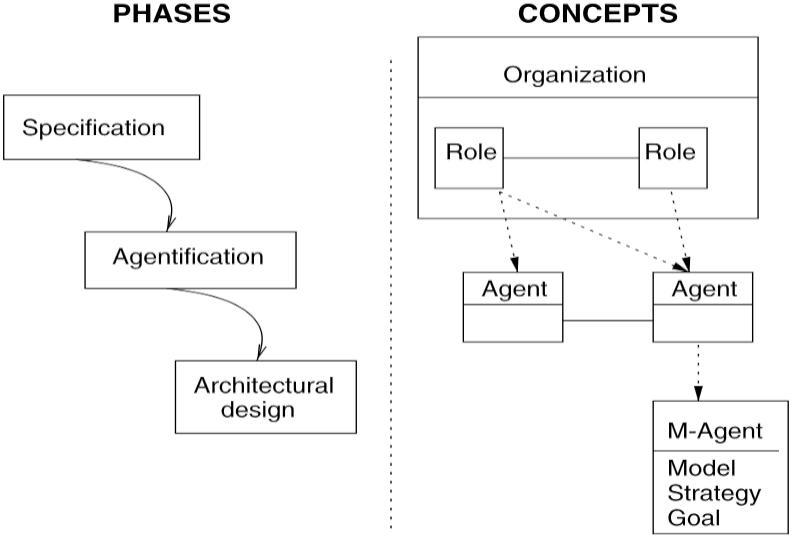
\includegraphics[width=\linewidth]{fig/RIO approach.png}
        \caption{Proces rozwoju w~metodologii RIO. (źródło: A formal framework for multi-agent systems analysis and design~\cite{S095741740200070220020101})}
        \label{fig:rio}
    \end{figure}

    System jest postrzegany jako organizacja która składa się ze zbioru wchodzących w~interakcję ról.
    Role złożone powinny być dekomponowane na~prostsze.
    Proces projektowania, przedstawiony na~rysunku~\ref{fig:rio}, składa się z~dwóch etapów: agentyfikacji i~projektowania architektonicznego.
    Agentyfikacja to~przypisanie roli do~agentów.
    Na~tym etapie nie robi się założeń co~do~architektury agentów.
    Dopiero etap projektowania architektonicznego kładzie naciska na~wewnętrzną architekturę agenta.

    \subsection{Metodologia Gaia}
    Metodologia analizy i~projektowania systemu agentowego Gaia, opisana w~pracy~\cite{Wooldridge2000a},
    została założona na~bazie widzenia systemu wieloagentowego jako organizacji obliczeniowej składającej się z~wielu oddziałujących ze sobą ról.
    Proces analizy i~projektowania, przedstawiony na~rysunku~\ref{fig:gaia}, może być postrzegany
    jako przyrostowe budowanie coraz bardziej złożonych modeli systemu, który ma być stworzony.

    \begin{figure}[!ht]
        \centering
        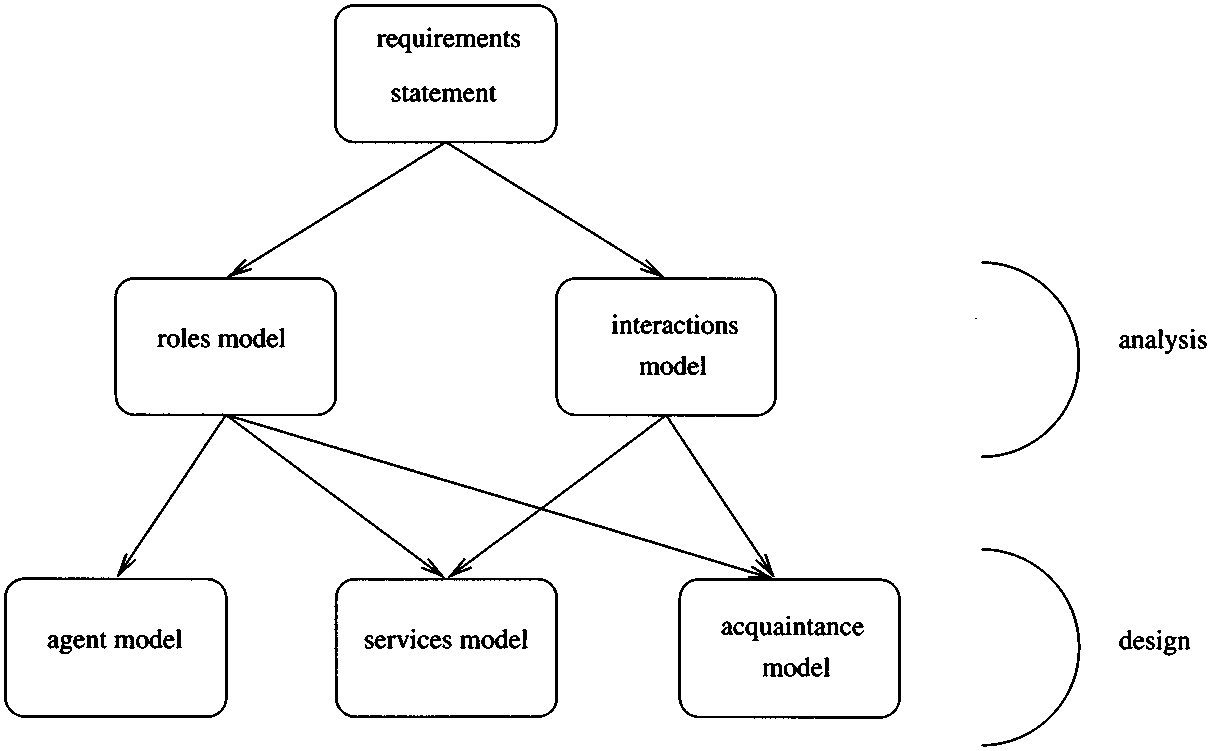
\includegraphics[width=\linewidth]{fig/gaia models.png}
        \caption{Związek pomiędzy modelami Gaia. (źródło: The Gaia Methodology for Agent-Oriented Analysis and Design~\cite{Wooldridge2000a})}
        \label{fig:gaia}
    \end{figure}

    Celem etapu analizy jest rozwinięcie zrozumienia systemu i~jego struktury.
    Podczas etapu projektowania Gaia skupia się na~tym jak agenci mają kooperować aby zrealizować cele systemu oraz czego wymaga się od~każdego agenta, aby to~osiągnąć.

    \subsection{Metodologia Gaia w~wersji 2}
    GAIA v2~\cite{Zambonelli2003} jest oficjalnym rozszerzeniem metodologii.
    Role i~protokoły są uzupełnione o~środowisko, w~którym działają agenci, specyfikujące jednostki i~zasoby.
    Dodatkowe abstrakcje organizacyjne zostały przedstawione na~rysunku~\ref{fig:gaia_v2}.

    \begin{figure}[!ht]
        \centering
        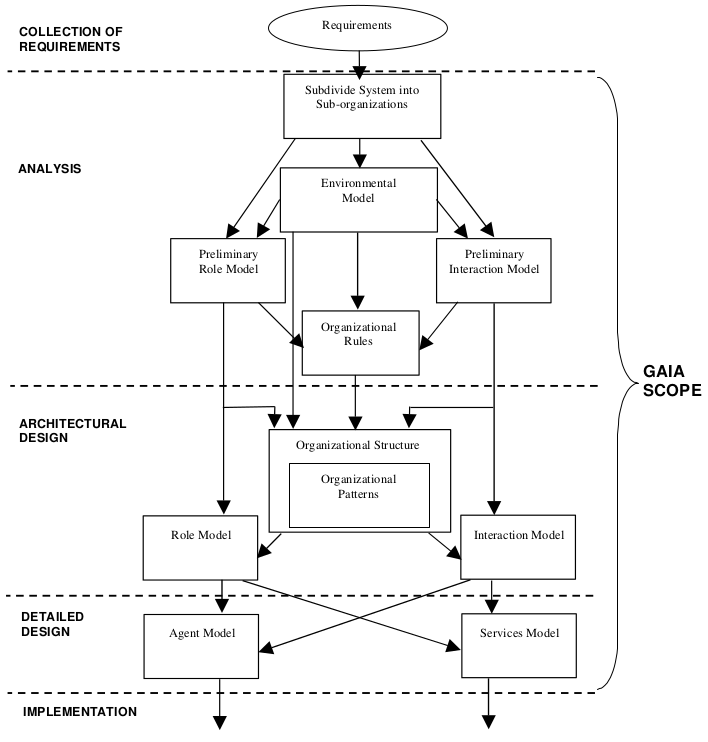
\includegraphics[width=\linewidth]{fig/gaia2 models.png}
        \caption{Modele i~związki w~GAIA v2. (źródło: Developing Multiagent Systems: The Gaia Methodology~\cite{Zambonelli2003})}
        \label{fig:gaia_v2}
    \end{figure}

    Reguły organizacyjne to~ograniczenia które muszą być uwzględnione w~globalnym zachowaniu organizacji.
    Struktura organizacyjna określa ogólną architekturę systemu.

    \subsection{Rozszerzenie metodologi Gaia - ROADMAP}
    ROADMAP~\cite{Juan2002a} jest kolejnym rozszerzeniem metodologii GAIA\@.
    Faza analizy jest rozszerzona tak by pokryć również specyfikację.
    Wprowadzono dodatkowe modele opisujące środowisko oraz wiedzę agentów.
    Rysunek~\ref{fig:roadmap} przedstawia strukturę modeli ROADMAP\@.

    \begin{figure}[!ht]
        \centering
        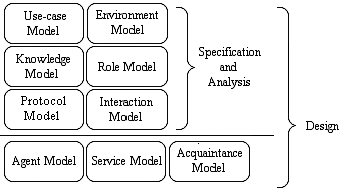
\includegraphics[width=\linewidth]{fig/roadmap models.png}
        \caption{Struktura modeli ROADMAP. (źródło: ROADMAP: Extending the Gaia methodology for complex open systems~\cite{Juan2002a})}
        \label{fig:roadmap}
    \end{figure}

    Hierarchia ról pełni podobną role do~struktury i~ról organizacyjnych w~GAIA v2.
    Pozwala określić właściwe zachowanie agentów.

    \subsection{Metodologia INGENIAS}
    Metodologię rozwoju systemu wieloagentowego INGENIAS autorzy przedstawili w~pracy pt.\@ ``Agent oriented software engineering with INGENIAS''~\cite{Pavon2003}.
    Metodologia ta ostała zaprojektowana z~myślą o~budowie specyfikacji przyrostowo z~zapewnieniem poprawności rozwoju.
    INGENIAS ulepsza oryginalne podejście z~MESSAGE/UML poprzez dodanie nowego widoku oraz dostarczenie narzędzi do~generowania kodu i~dokumentacji systemu automatycznie ze specyfikacji.
    Generalnym podejściem INGENIAS do~specyfikacji systemu wieloagentowego jest podział problemu na~aspekty, które tworzą różne widoki systemu.
    Każdy rodzaj widoku jest opisany z~wykorzystaniem języka meta-modelującego.
    INGENIAS wyróżnia pięć metamodeli opisujących widoki, które muszą zostać wykorzystane przy opisie systemu:
    \begin{enumerate}
        \item Model agenta, który opisuje pojedynczego agenta, jego zadania, cele, początkowy stan oraz role,
        \item Model interakcji, który opisuje jakie interakcje mogą zajść między agentami,
        \item Model zadań i~celów, który opisuje relację między zadaniami i~celami oraz ich strukturami,
        \item Model organizacji, który opisuje jak komponenty systemu są ze sobą pogrupowane, jakie ograniczenia istnieją w~interakcjach między agentami,
        \item Model środowiska, który definiuje postrzeganie agentów jako elementów systemu oraz identyfikuje zasoby systemu.
    \end{enumerate}


    \section{Fuzja wiedzy}

    Technologia systemów wieloagentowych jako podstawa systemów Fuzji Wiedzy została przedstawiona w~pracy z~2001 roku~\cite{Smirnov2002}.
    Fuzje Wiedzy można zdefiniować jako integrację luźno powiązanych źródeł, w~połączone zasoby, w~celu uzupełnienia niedostatecznej wiedzy i~uzyskania nowej.
    Korzystanie z~inteligentnych agentów zwiększa wydajność i~interoperacyjność systemu, ponieważ agenci mogą działać w~środowisku rozproszonym,
    niezależnie od~użytkownika, i~wykorzystywać ontologie do~reprezentacji i~wymiany wiedzy.


    \chapter{Koncepcja}\label{ch:koncepcja}
    System Agentowy zajmuje się analizą danych znajdujących się w~bazie GDELT\@.
    Identyfikowane są wzorce opisujące państwa oraz relacje między nimi.
    Stworzone reguły wspomagają odnajdywanie wzorców.

    Wejściem systemu jest zadanie konfiguracyjne.
    Zadanie konfiguracyjne uruchamia system który szuka wzorców.
    Działanie systemu przebiega wg następujących punktów:
    \begin{enumerate}
        \item rozdział zadań dla agentów,
        \item wyszukiwanie wzorców,
        \item zbieranie danych,
        \item analiza,
        \item generowanie zestawień.
    \end{enumerate}

    Grupy agentów profilowane są w~celu automatycznego wyszukiwania wzorców czasowych.
    Zróżnicowanie agentów obejmuje:
    \begin{enumerate}
        \item progi,
        \item poziomy granulacji,
        \item wyszukiwanie korelacji,
        \item wyszukiwanie trendów.
    \end{enumerate}

    Na~wyjściu systemu otrzymujemy zagregowane dane.


    \section{Wybór wzorców}\label{sec:wybór-wzorców}


    W wersji podstawowej systemu, na~podstawie danych zgromadzonych w~bazie danych GDELT będą wyszukiwane wzorce:
    \begin{itemize}
        \item symetria siły połączenia
        \item mocarstwo-klient
    \end{itemize}


    \section{Role i~Interakcje}

    \subsection{Role}
    Rola agenta określa, czego oczekuje się od~niego zarówno w~porozumieniu z~innymi agentami, jak i~w~odniesieniu do~całego systemu.
    Często rola agenta jest po prostu definiowana w~kategoriach konkretnego zadania, które ma on wykonać w~kontekście systemu.
    W metodologii GAIA rola jest definiowana przez cztery atrybuty~\cite{Wooldridge2000a}:
    \begin{enumerate}
        \item obowiązki,
        \item uprawnienia,
        \item aktywności,
        \item protokoły.
    \end{enumerate}
    Obowiązki determinują funkcjonalność i~są podzielone na~dwa typy:
    \begin{enumerate}
        \item właściwości żywotności - opisują te stany które agent musi wywołać, coś zostanie zrobione,
        \item właściwości bezpieczeństwa - sprawdzają po każdym wykonaniu czy~stan jest akceptowalny.
    \end{enumerate}
    Uprawnienia to~prawa związane z~rolą.
    Identyfikują zasoby które sa dostępne dla danej roli w~celu realizacji obowiązków.
    Działania to~obliczenia związane z~rolą, które mogą być przeprowadzone przez agenta bez interakcji z~innymi.
    Protokoły definiują sposób w~jaki role wchodzą w~interakcję ze sobą.

    W Systemie zostały przewidziane następujące role:

    \begin{enumerate}
        \item Poszukiwacz wzorców~\ref{tab:schemat roli Poszukiwacz Wzorców}
        \begin{enumerate}
            \item Poszukiwacz wzorców w~danych GDELT
            \begin{enumerate}
                \item Poszukiwacz Wzorców Statycznych
                \begin{enumerate}
                    \item symetria
                    \item mocarstwo-klient
                \end{enumerate}
            \end{enumerate}
        \end{enumerate}
        \item Poszukiwacz Korelacji~\ref{tab:schemat roli poszukiwacz korelacji}
        \item Generator Zestawień~\ref{tab:schemat roli Generator Zestawień}
    \end{enumerate}

    \begin{table}[ht!]
        \begin{tabular}{ll}
            Schemat roli:          & PoszukiwaczKorelacji                                           \\ \hline
            Opis                   & Ta rola obejmuje wyszukiwanie korelacji między krajami         \\
            & na~podstawie danych pobranych od~poszukiwaczy wzorców.         \\
            Protokoły i~Aktywności & \textbf{sprawdzajWzorce, szukajKorelacji, poinformujGenerator} \\
            Uprawnienia            & \textbf{czyta dostarczone} \textit{PoszukiwaczWzorców}         \\
            & ~~~~~~\textit{wzorzec}                                         \\
            & \textbf{zmienia} \textit{zestawienie}                          \\
            Obowiązki              &                                                                \\
            ~~żywotność            & \textbf{sprawdzajWzorce, szukajKorelacji, poinformujGenerator} \\
            ~~bezpieczeństwo       & -                                                              \\
        \end{tabular}
        \caption{Schemat roli Poszukiwacz Korelacji. (źródło: Opracowanie własne)}
        \label{tab:schemat roli poszukiwacz korelacji}
    \end{table}

    \begin{table}[ht!]
        \begin{tabular}{ll}
            Schemat roli:          & Generator Zestawień                                                          \\ \hline
            Opis                   & Ta rola obejmuje tworzenie zestawień na~podstawie                            \\
            & danych zebranych przez poszukiwaczy korelacji i~trendów.                     \\
            Protokoły i~Aktywności & \textbf{sprawdzajZestawienia}                                                \\
            Uprawnienia            & \textbf{czyta dostarczone} \textit{PoszukiwaczKorelacji, PoszukiwaczTrendów} \\
            & ~~~~~~\textit{zestawienie}                                                   \\
            & \textbf{zmienia} \textit{zestawienie}                                        \\
            Obowiązki              &                                                                              \\
            ~~żywotność            & \textbf{sprawdzajZestawienia}                                                \\
            ~~bezpieczeństwo       & -                                                                            \\
        \end{tabular}
        \caption{Schemat roli Generator Zestawień. (źródło: Opracowanie własne)}
        \label{tab:schemat roli Generator Zestawień}
    \end{table}

    \begin{table}[ht!]
        \begin{tabular}{ll}
            Schemat roli:          & Poszukiwacz Wzorców                             \\ \hline
            Opis                   & Ta rola obejmuje wyszukiwanie wzorców           \\
            & pośród danych z~wykorzystaniem zestawu miar.    \\
            & Wzorce dzielą się na~dwie kategorie: wewnętrzne \\
            & oraz między krajami.                            \\
            Protokoły i~Aktywności & \textbf{SzukajWzorców}                          \\
            Uprawnienia            & \textbf{czyta} \textit{miary}                   \\
            & \textbf{zmienia} \textit{wzorzec}               \\
            Obowiązki              &                                                 \\
            ~~żywotność            & \textbf{SzukajWzorców}                          \\
            ~~bezpieczeństwo       & -                                               \\
        \end{tabular}
        \caption{Schemat roli Poszukiwacz Wzorców. (źródło: Opracowanie własne)}
        \label{tab:schemat roli Poszukiwacz Wzorców}
    \end{table}

    \subsection{Interakcje}
    W systemie zamkniętym wszyscy agenci są znani a~priori i~mają ze sobą współpracować, a~zatem mogą sobie ufać podczas interakcji.
    W metodologii GAIA model interakcji składa się ze zbioru definicji protokołów.
    Protokół to~wzorzec interakcji który został formalnie zdefiniowany i~wyodrębniony.

    Interakcje wyodrębnione w~Systemie to:

    \begin{enumerate}
        \item zgłoszenie znalezionej informacji przez agenta szukającego wzorców do~agenta poszukującego korelacji i~trendów,
        \item przekazanie informacji do~agenta generującego zestawienia.
    \end{enumerate}

    \subsection{Agenci}
    Zadanie konfiguracyjne określa na~jakich krajach będzie skupiona uwaga systemu.
    Pojedynczy agent pełni rolę Generatora Zestawień, który tworzy Poszukiwaczy Korelacji.
    Poszukiwacze Korelacji tworzą Poszukiwaczy Wzorców którzy przetwarzają dane pobrane z~GDELT\@.


    \section{Współdziałanie agentów}
    Na~rysunku~\ref{fig:relacje} przedstawiony został schemat współdziałania agentów.

    \begin{figure}[!ht]
        \centering
        \includegraphics[width=\linewidth]{fig/relacja ról.png}
        \caption{Interakcje ról. (źródło: Opracowanie własne)}
        \label{fig:relacje}
    \end{figure}


    \chapter{Realizacja}\label{ch:realizacja}


    \section{Wybór systemu agentowego}

    W języku Python istnieje wiele bibliotek do~analizy danych oraz uczenia maszynowego.
    Aby uniknąć potrzeby generowania powiązań z~innymi językami wybrano platformę agentową również w~języku Python.
    W tabeli~\ref{tab:porownanie} zebrane zostały cechy wybranych platform w~tym języku.


    \begin{table}[tbp]
        \begin{tabular}{l|ll}
            & SPADE                                   & PADE                     \\ \hline
            komunikacja            & serwer XMPP                             & biblioteka Twisted       \\
            & FIPA, XMPP Data Forms~\cite{data_forms} & FIPA ACL~\cite{fipa_acl} \\ \hline
            filtrowanie wiadomości & metadane                                & klasa filtrująca         \\ \hline
            licencja               & MIT                                     & MIT                      \\ \hline
            transfer               & zserializowani agenci                   & agenci mogą być          \\
            &                                         & zawartością wiadomości   \\ \hline
            zachowania             & wiele jednocześnie:                     & cykliczne i~periodyczne  \\
            & cykliczne i~periodyczne \\ \hline
            obecność kontaktów     & powiadomienia                           & -                        \\
            & w~czasie rzeczywistym \\ \hline
            interfejs graficzny    & webowy                                  & webowy (Flask)           \\ \hline
            rozszerzenia           & wtyczki                                 & -                        \\ \hline \hline
        \end{tabular}
        \caption{Porównanie wybranych platform wieloagentowych w~języku python. (źródło: opracowanie własne)}
        \label{tab:porownanie}
    \end{table}

    \subsection{Mesa}
    Mesa~\cite{Masad2015} to~biblioteka do~modelowania agentowego w~Pythonie.
    Pozwala na~szybkie stworzenie modelu agentowego przy wykorzystaniu wbudowanych komponentów
    Ostatnie zmiany wprowadzone w~tej bibliotece, na~jej stronie w~serwisie GitHub \href{https://github.com/projectmesa/mesa}{Project~Mesa~github}, są datowane na~11 lutego 2021 (stan na~17 II 2021r.).

    \subsection{Python Agent DEvelopment framework}
    Framework PADE~\cite{Melo2019} umożliwia rozwój, wykonanie i~zarządzanie wieloagentowymi systemami w~rozproszonym środowisku.
    Najnowsza aktualizacja tego frameworku, w~serwisie GitHub~\href{https://github.com/grei-ufc/pade}{Smart~Grids~Research~Group~-~UFC~github} pochodzi z~4 lutego 2021 (stan na~17 II 2021r.).

    \subsection{Smart Python multi-Agent Development Environment}
    Platforma wieloagentowa SPADE jest oparta o~XMPP\cite{Saint-Andre2007}.
    Aktualna modyfikacja tej platformy, w~serwisie GitHub~\href{https://github.com/javipalanca/spade}{javipalanca~github}, pochodzi z~22~maja 2020 (stan na~17 II 2021r.).
%    powiększa stronę aby część zdania nie trafiła pod~rysunek
    \enlargethispage{1\baselineskip}

    \subsection{Podsumowanie}
    Do wykonania systemu wybrany został framework SPADE\@.
    Pomimo tego, że poprawki w~tej platformie wprowadzane są rzadziej niż w~PADE, to~zawiera ona dużo bogatszą dokumentację
    oraz liczne przykłady użycia, co~znacznie obniża próg wejścia do~budowy systemu agentowego.


    \section{Analiza zdarzeń wewnętrznych USA}
    W tej sekcji przedstawiona została analiza zdarzeń wewnętrznych (takich w~których jest ten sam pierwszy i~drugi aktor) w~Stanach Zjednoczonych.
    To badanie ma na~celu wykazanie czy~podczas analizy krajów i~relacji rozdzielane powinny być zdarzenia wewnętrzne oraz zewnętrzne.

    \subsection{Kody bazowe (Event Base Codes)}\label{subsec:kody-bazowenullevent-base-codesnull}

    Liczba zdarzeń wewnętrznych \textit{Make a~visit} w~USA w~latach 2015-2020 to~około 810 tysięcy.
    Zdarzeń zewnętrznych \textit{Make a~visit} w~USA w~tym okresie było 3 razy więcej - około 2,4 miliona,
    podczas gdy globalna liczba zdarzeń \textit{Make a~visit} wynosiła około 41 milionów.

    Na~wykresach zostało przedstawionych 20 najliczniejszych Kodów bazowych.

    Porównanie wykresów z~kodami bazowymi przedstawiających liczbę zdarzeń:
    \begin{itemize}
        \item wewnętrznych w~USA~\ref{fig:USA_inner_EBC},
        \item pomiędzy USA i~innymi krajami~\ref{fig:USA_not_inner_EBC},
        \item globalnie~\ref{fig:GLOBAL_EBC},
    \end{itemize}
    wykazuje podobieństwo.

    \begin{figure}[tp]
        \centering
        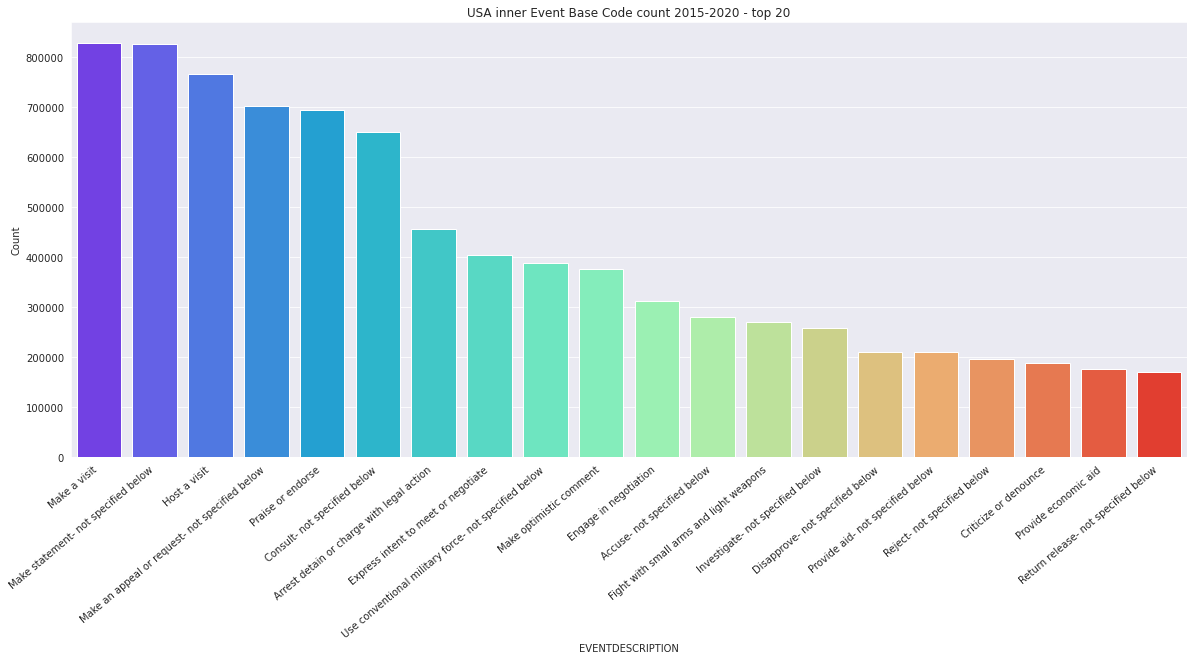
\includegraphics[width=\linewidth]{fig/USA inner/EBC.png}
        \caption{Liczba zdarzeń wewnętrznych USA dla kodów bazowych od~2015 - top 20. (źródło: opracowanie własne)}
        \label{fig:USA_inner_EBC}
    \end{figure}


    \begin{figure}[tp]
        \centering
        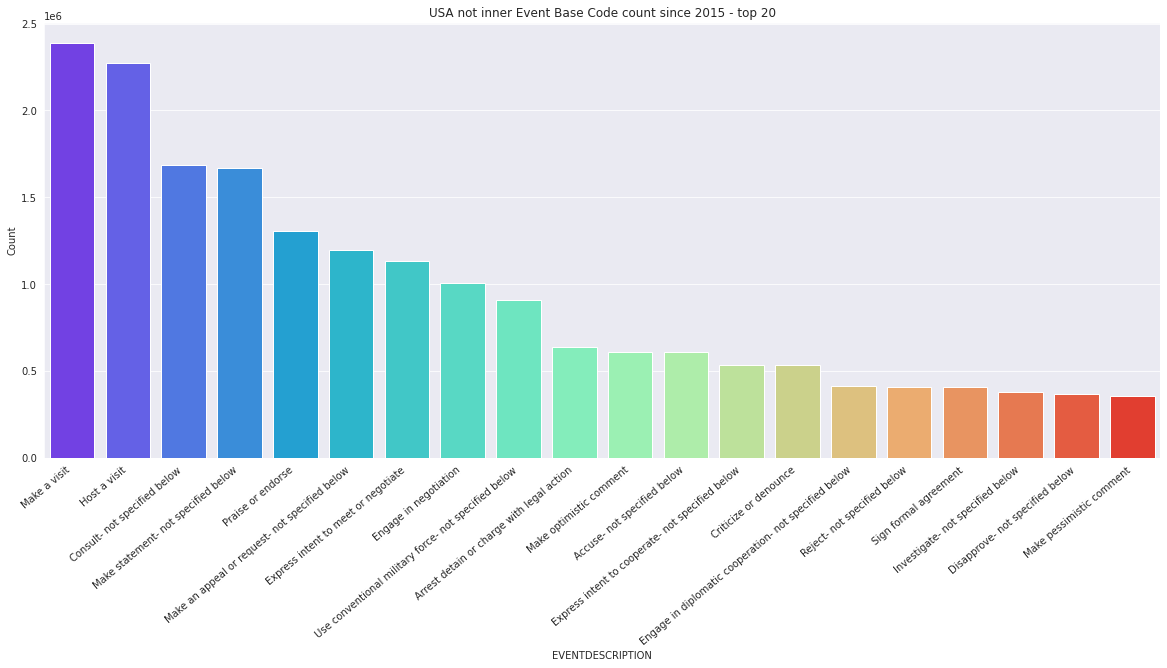
\includegraphics[width=\linewidth]{fig/USA not inner/EBC.png}
        \caption{Liczba zdarzeń zewnętrznych USA dla kodów bazowych od~2015 - top 20. (źródło: opracowanie własne)}
        \label{fig:USA_not_inner_EBC}
    \end{figure}

    \begin{figure}[tp]
        \centering
        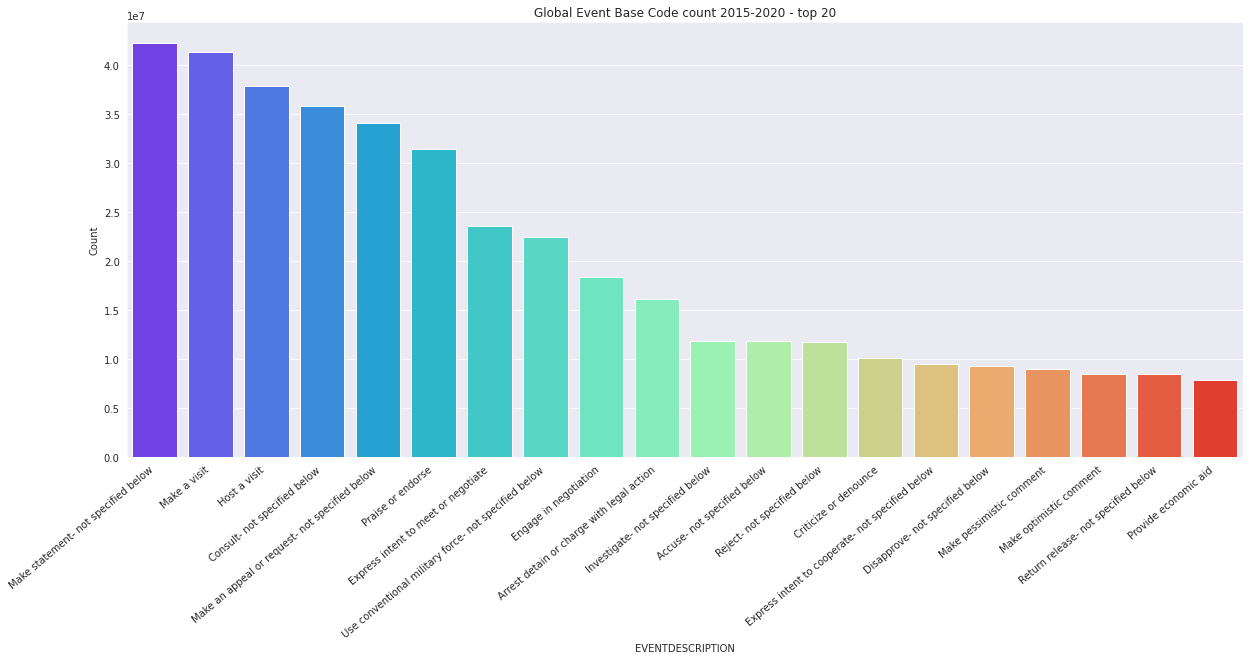
\includegraphics[width=\linewidth]{fig/GLOBAL//EBC.png}
        \caption{Liczba zdarzeń dla kodów bazowych od~2015 - top 20. (źródło: opracowanie własne)}
        \label{fig:GLOBAL_EBC}
    \end{figure}

    Procentowe udziały zdarzeń wewnętrznych i~zewnętrznych USA oraz globalnych, w~latach 2015-2020, zostały przedstawione
    w~dodatku~\ref{subsec:kody-bazowenullevent-base-codesnull2}.

    Zarówno dla zdarzeń wewnętrznych USA, jak i~globalnych w~pierwszej trójce występują zdarzenia:
    \begin{itemize}
        \item \textit{Make a~visit},
        \item \textit{Make statement - not specific below},
        \item \textit{Host a~visit}.
    \end{itemize}
    Dla zdarzeń zewnętrznych USA w~pierwszej trójce \textit{Make statement - not specific below} zostaje zastąpione przez \textit{Consult - not specific below}.
    \textit{Make statement - not specific below} pojawia się na~4 pozycji.

    Takie wyniki mogą świadczyć o~podobieństwie klasyfikacji bazowej (Base Codes) zdarzeń,
    niezależnie od~tego czy~są to~zdarzenia wewnętrzne czy~zewnętrzne.

    \subsection{Kody podstawowe (Event Root Codes)}\label{subsec:kody-podstawowenullevent-root-codesnull}

    Podobnie jak w~przypadku kodów bazowych, porównanie wykresów z~kodami bazowymi przedstawiających liczbę zdarzeń:
    \begin{itemize}
        \item wewnętrznych w~USA~\ref{fig:USA_inner_ERC},
        \item pomiędzy USA i~innymi krajami~\ref{fig:USA_not_inner_ERC},
        \item globalnie~\ref{fig:GLOBAL_ERC},
    \end{itemize}
    wykazuje podobieństwo.

    \begin{figure}[tp]
        \centering
        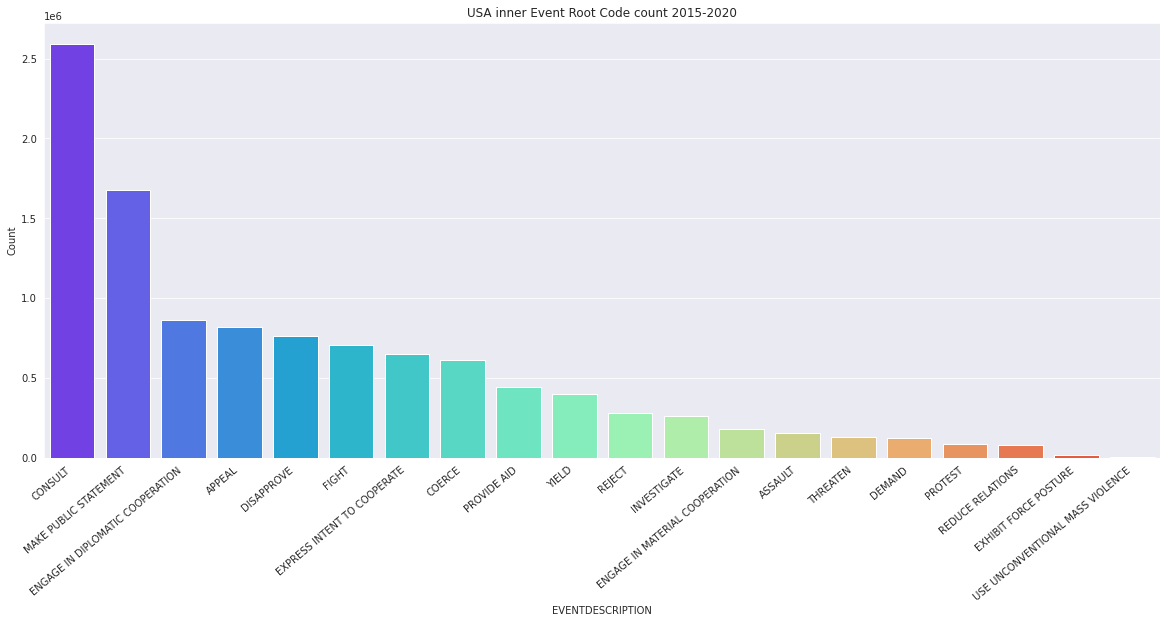
\includegraphics[width=\linewidth]{fig/USA inner/ERC.png}
        \caption{Liczba zdarzeń wewnętrznych USA dla wszystkich kodów podstawowych od~2015. (źródło: opracowanie własne)}
        \label{fig:USA_inner_ERC}
    \end{figure}

    \begin{figure}[tp]
        \centering
        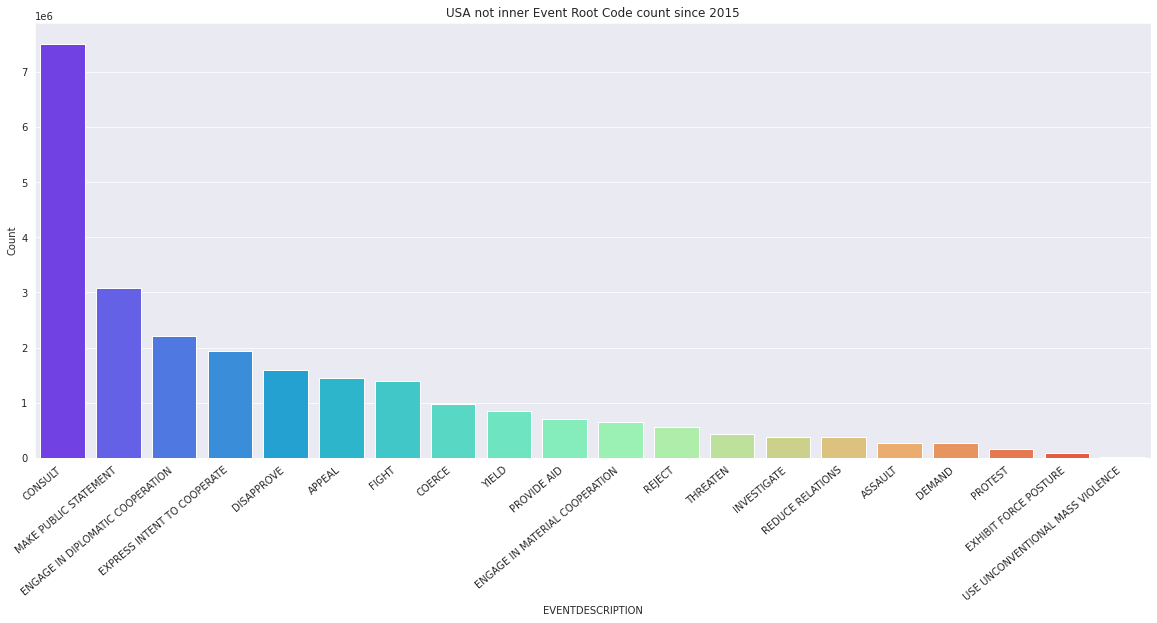
\includegraphics[width=\linewidth]{fig/USA not inner/ERC.png}
        \caption{Liczba zdarzeń zewnętrznych USA dla kodów podstawowych od~2015 - top 20. (źródło: opracowanie własne)}
        \label{fig:USA_not_inner_ERC}
    \end{figure}

    \begin{figure}[tp]
        \centering
        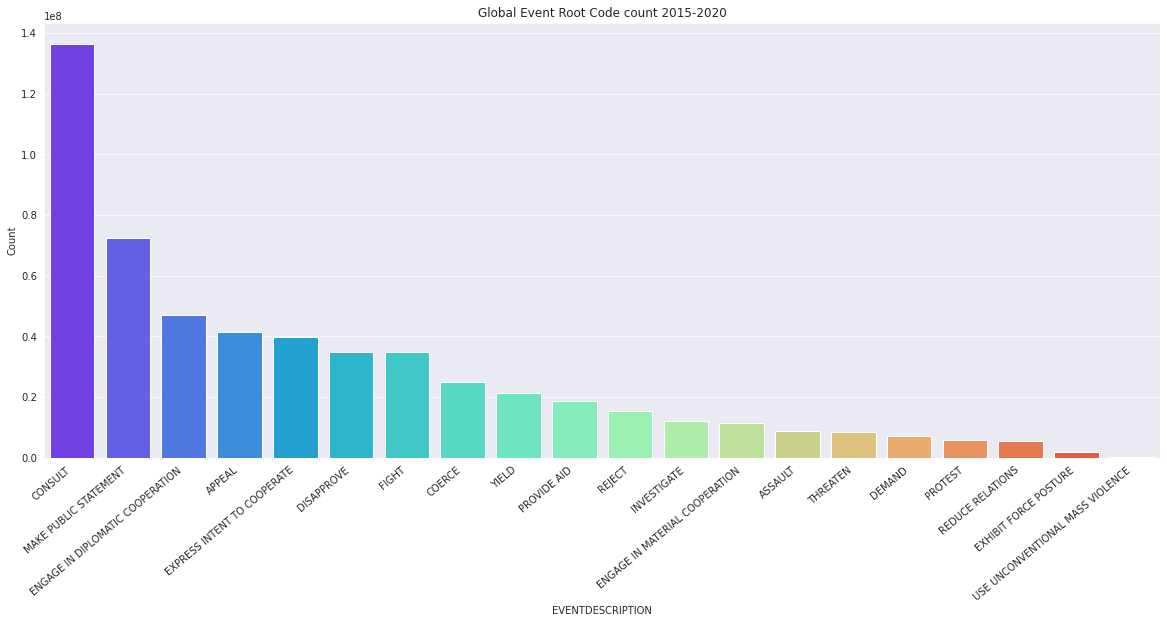
\includegraphics[width=\linewidth]{fig/GLOBAL//ERC.png}
        \caption{Liczba zdarzeń dla kodów podstawowych od~2015 - top 20. (źródło: opracowanie własne)}
        \label{fig:GLOBAL_ERC}
    \end{figure}

    Procentowe udziały zdarzeń wewnętrznych i~zewnętrznych USA oraz globalnych, w~latach 2015-2020, zostały przedstawione
    w~dodatku~\ref{subsec:kody-podstawowenullevent-root-codesnull2}.

    Liczba zdarzeń wewnętrznych \textit{Consult} w~USA w~latach 2015-2020 to~około 2,5 miliona.
    Zdarzeń zewnętrznych \textit{Consult} w~USA w~tym okresie było 3 razy więcej - około 7,5 miliona,
    podczas gdy globalna liczba zdarzeń \textit{Consult} wynosiła około 140 milionów.

    Zarówno dla zdarzeń wewnętrznych USA, zewnętrznych USA jak i~globalnych pierwsza trójka wygląda następująco:
    \begin{enumerate}
        \item \textit{Consult},
        \item \textit{Make public statement},
        \item \textit{Engage in diplomatic cooperation}.
    \end{enumerate}

    Takie wyniki wyraźnie świadczą o~podobieństwie klasyfikacji podstawowej (Root Codes) zdarzeń.

    \subsection{Czterokody (Quad Class)}\label{subsec:czterokodynullquad-classnull}

    W najwyższym poziomie agregacji typu zdarzeń przy porównaniu wykresów z~kodami bazowymi przedstawiających liczbę zdarzeń:
    \begin{itemize}
        \item wewnętrznych w~USA~\ref{fig:USA_inner_QC},
        \item pomiędzy USA i~innymi krajami~\ref{fig:USA_not_inner_QC},
        \item globalnie~\ref{fig:GLOBAL_QC},
    \end{itemize}
    obserwujemy największe podobieństwo.

    \begin{figure}[tp]
        \centering
        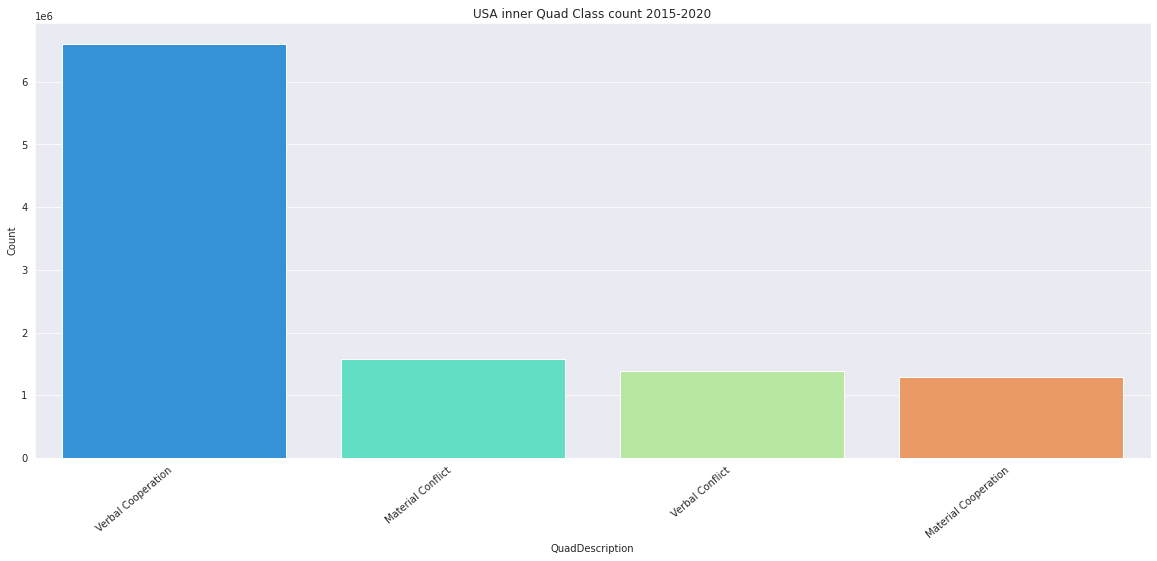
\includegraphics[width=\linewidth]{fig/USA inner/QC.png}
        \caption{Liczba zdarzeń wewnętrznych USA dla czterokodów od~2015. (źródło: opracowanie własne)}
        \label{fig:USA_inner_QC}
    \end{figure}


    \begin{figure}[tp]
        \centering
        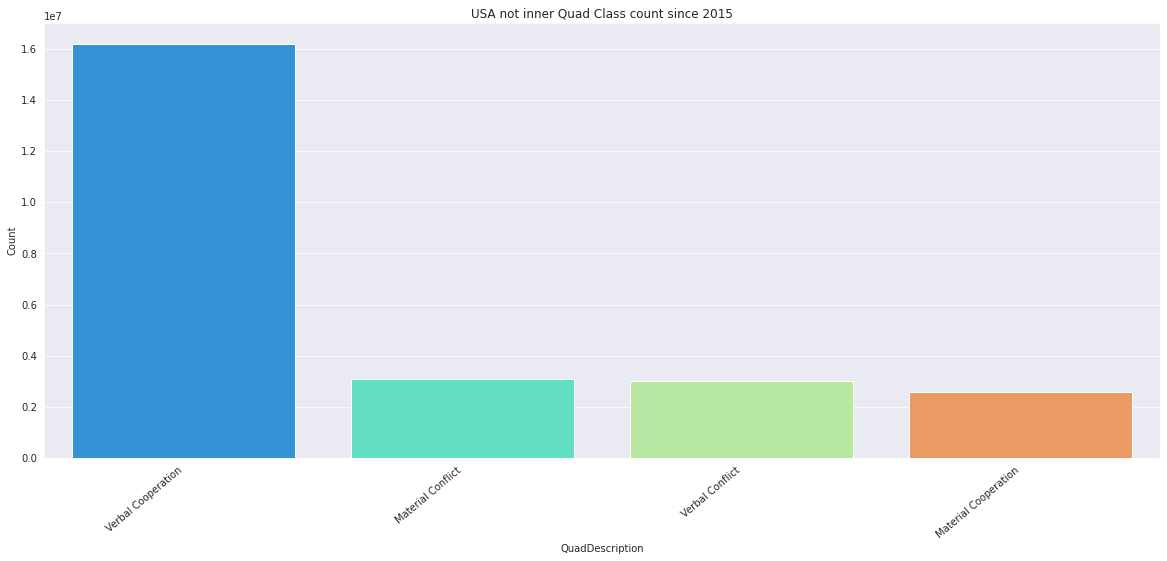
\includegraphics[width=\linewidth]{fig/USA not inner/QC.png}
        \caption{Liczba zdarzeń zewnętrznych USA dla kodów podstawowych od~2015 - top 20. (źródło: opracowanie własne)}
        \label{fig:USA_not_inner_QC}
    \end{figure}


    \begin{figure}[tp]
        \centering
        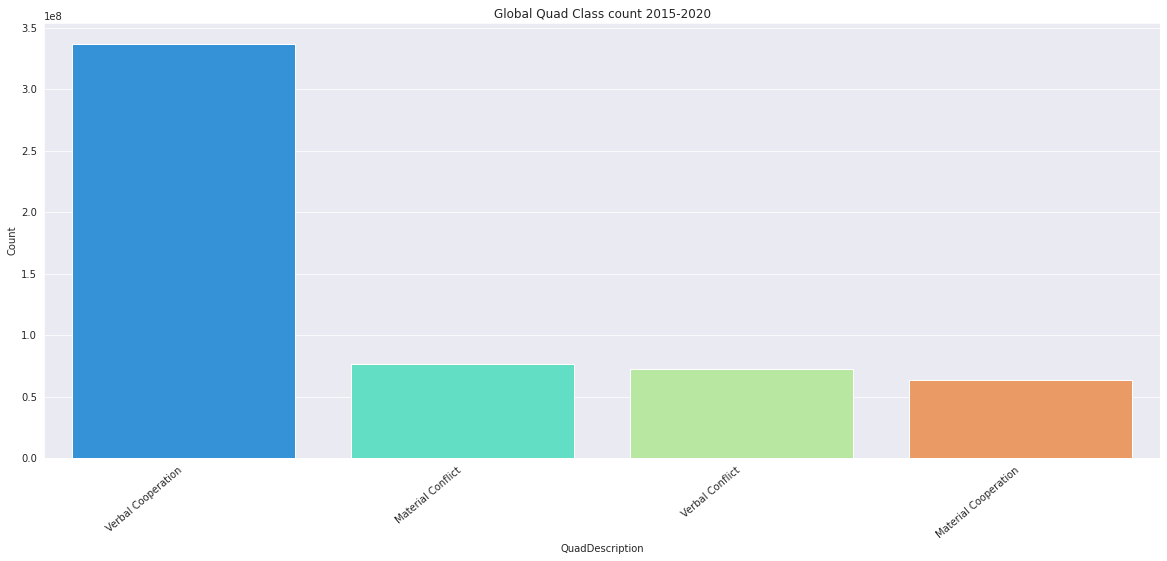
\includegraphics[width=\linewidth]{fig/GLOBAL//QC.png}
        \caption{Liczba zdarzeń dla kodów podstawowych od~2015 - top 20. (źródło: opracowanie własne)}
        \label{fig:GLOBAL_QC}
    \end{figure}

    Procentowe udziały zdarzeń wewnętrznych i~zewnętrznych USA oraz globalnych, w~latach 2015-2020, zostały przedstawione
    w~dodatku~\ref{subsec:czterokodynullquad-classnull2}.

    Liczba zdarzeń wewnętrznych \textit{Verbal Cooperation} w~USA w~latach 2015-2020 to~około 6,5 miliona.
    Zdarzeń zewnętrznych \textit{Verbal Cooperation} w~USA w~tym okresie było 3 razy więcej - około 16 milionów,
    podczas gdy globalna liczba zdarzeń \textit{Verbal Cooperation} wynosiła około 340 milionów.

    Dla wszystkich typów zdarzeń czterokody występują w~następującej kolejności:
    \begin{enumerate}
        \item \textit{Verbal Cooperation},
        \item \textit{Material Conflict},
        \item \textit{Verbal Conflict},
        \item \textit{Material Cooperation}.
    \end{enumerate}
    Dla każdego typu zdarzeń przeważającą większość stanowią zdarzenia \textit{Verbal Cooperation}.

    Takie wyniki wyraźnie świadczą o~podobieństwie przyporządkowań zdarzeń do~czterokodów (Quad Class).

    \subsection{Podsumowanie}
    Przeprowadzona analiza pokazuje duże podobieństwo pomiędzy zdarzeniami wewnętrznymi i~zewnętrznymi dla USA oraz globalnymi.
    Pozwala to~przypuszczać, że podobna zależność występuje dla pozostałych krajów.
    Z tego powodu, w~dalszych pracach, zdarzenia wewnętrzne nie będą osobno rozważane.


    \section{Analiza Power-Client}\label{sec:analiza-power-client}
    W tej części przedstawione zostaną wyniki wstępnej analizy mającej na~celu wyłonienie miar
    do~poszukiwań wzorca Power-Client.

    Dla Kodów głównych jak i~Kodów bazowych pierwsza analiza została przeprowadzona w~trzech wersjach:
    \begin{itemize}
        \item bez progowania,
        \item z~progiem skali Goldsteina >= 3,
        \item z~progiem liczby wzmianek >= 5.
    \end{itemize}
    Wybrane zostały następujące pary krajów:
    \begin{itemize}
        \item jako przykład relacja klient-hegemon:
        \begin{itemize}
            \item Polska-USA,
            \item Polska-Rosja,
            \item Polska-Niemcy,
        \end{itemize}
        \item jako przykład relacji neutralnych:
        \begin{itemize}
            \item Polska-Hiszpania,
            \item Polska-Czechy,
            \item Polska-Węgry.
        \end{itemize}
    \end{itemize}

    Jeśli wyniki były zadowalające - wyraźna różnica pomiędzy układem zdarzeń - to~tworzone zostały wykresy podsumowujące.
    Na~ostatnim etapie z~wykresów podsumowujących wybierane były ręcznie te, zawierające przynajmniej 8 krajów, na~których była widoczna najlepsza separacja relacji klient-hegemon od~relacji neutralnych.
    Kryterium wyboru była zauważalna separacja relacji klient-hegemon oraz neutralnych.

    \subsection{Event Root Code}\label{subsec:event-root-code}

    \subsubsection{Bez progowania}

    \begin{figure}[tp]
        \centering
        \includegraphics[width=\linewidth]{../Power-Client pre analysis/fig_EventRootCode/POL-USA EventRootCode count 2015-2020 - top 20.png}
        \caption{Procentowa liczba zdarzeń POL-USA wg kodów głównych. (źródło: opracowanie własne)}
        \label{fig:Power-Client:ERC:POL-USA}
    \end{figure}

    \begin{figure}[tp]
        \centering
        \includegraphics[width=\linewidth]{../Power-Client pre analysis/fig_EventRootCode/POL-ESP EventRootCode count 2015-2020 - top 20.png}
        \caption{Procentowa liczba zdarzeń POL-ESP wg kodów głównych. (źródło: opracowanie własne)}
        \label{fig:Power-Client:ERC:POL-ESP}
    \end{figure}

    Zarówno w~przypadku relacji Polska-USA (wykres~\ref{fig:Power-Client:ERC:POL-USA}) jak i~Polska-Hiszpania (wykres~\ref{fig:Power-Client:ERC:POL-ESP})
    na~pierwszym miejscu występują zdarzenia \textit{CONSULT}.

    Pozostałe wykresy zostały dołączone w~sekcji~\ref{subsubsec:erc:bez-progowania}.

    Na~każdym z~6 wykresów, niezależnie od~typu relacji, dominuje liczba zdarzeń \textit{CONSULT}.
    Dla relacji POL-USA oraz POL-RUS na~drugim miejscu są zdarzenia \textit{MAKE PUBLIC STATEMENT}.

    Taka obserwacja świadczy o~tym, że Kody główne bez progowania nie nadają się do~poszukiwania wzorca Power-Client.

    \subsubsection{Próg skala Goldsteina >=3}
    Skala Goldsteina przypisuje każdemu z~kodów CAMEO numeryczną wartość od~-10 do~10, przedstawia teoretyczny wpływ typu zdarzenia na~stabilność kraju.
    Ponieważ skala Goldsteina jest bezpośrednio związana z~kodem CAMEO, dlatego filtrowanie wg skali Goldsteina odrzuca cześć kodów.
    Kody CAMEO dla skali Goldsteina >=3 to:
    \begin{itemize}
        \item \textit{ENGAGE IN DIPLOMATIC COOPERATION}
        \item \textit{EXPRESS INTENT TO COOPERATE}
        \item \textit{APPEAL}
        \item \textit{CONSULT}
        \item \textit{YIELD}
        \item \textit{ENGAGE IN MATERIAL COOPERATION}
        \item \textit{PROVIDE AID}
        \item \textit{MAKE PUBLIC STATEMENT}
    \end{itemize}

    \begin{figure}[tp]
        \centering
        \includegraphics[width=\linewidth]{../Power-Client pre analysis/fig_EventRootCode/POL-USA EventRootCode count 2015-2020 with Goldstein Scale >=3 - top 20.png}
        \caption{Procentowa liczba zdarzeń POL-USA wg kodów głównych. (źródło: opracowanie własne)}
        \label{fig:Power-Client:ERC:Goldstein:POL-USA}
    \end{figure}


    \begin{figure}[tp]
        \centering
        \includegraphics[width=\linewidth]{../Power-Client pre analysis/fig_EventRootCode/POL-ESP EventRootCode count 2015-2020 with Goldstein Scale >=3 - top 20.png}
        \caption{Procentowa liczba zdarzeń POL-ESP wg kodów głównych. (źródło: opracowanie własne)}
        \label{fig:Power-Client:ERC:Goldstein:POL-ESP}
    \end{figure}

    Dla relacji Polska-USA (wykres~\ref{fig:Power-Client:ERC:Goldstein:POL-USA}) oraz Polska-Hiszpania (wykres~\ref{fig:Power-Client:ERC:Goldstein:POL-ESP})
    pierwsze cztery pozycje pod~względem procentowego udziału przedstawiają się w~następującej kolejności:
    \begin{itemize}
        \item \textit{ENGAGE IN DIPLOMATIC COOPERATION}.
        \item \textit{EXPRESS INTENT TO COOPERATE}.
        \item \textit{APPEAL}.
        \item \textit{CONSULT}.
    \end{itemize}

    Pozostałe wykresy zostały dołączone w~sekcji~\ref{subsubsec:erc:próg-skala-goldsteina->=3}.

    Na~każdym z~6 wykresów, niezależnie od~typu relacji, dominuje liczba zdarzeń \textit{ENGAGE IN DIPLOMATIC COOPERATION}.
    Dla wszystkich relacji, z~wyjątkiem POL-RUS, na~drugim miejscu są zdarzenia \textit{EXPRESS INTENT TO COOPERATE}.

    Powyższa analiza pokazuje, że Kody główne z~progowaniem skali Goldsteina >=3 nie nadają się do~poszukiwania wzorca Power-Client.

    \subsubsection{Próg ilość wzmianek >=5}
    Liczba wzmianek to~całkowita liczba wystąpień informacji o~danym zdarzeniu pośród dokumentów źródłowych.
    Pozwala określić ważność danego zdarzenia.
    Im więcej dyskusji o~danym zdarzeniu, tym bardziej prawdopodobne, że jest ono istotne.

    \begin{figure}[tp]
        \centering
        \includegraphics[width=\linewidth]{../Power-Client pre analysis/fig_EventRootCode/POL-USA EventRootCode count 2015-2020 with mentions >=5 - top 20.png}
        \caption{Procentowa liczba zdarzeń POL-USA wg kodów głównych. (źródło: opracowanie własne)}
        \label{fig:Power-Client:ERC:Mentions:POL-USA}
    \end{figure}

    \begin{figure}[tp]
        \centering
        \includegraphics[width=\linewidth]{../Power-Client pre analysis/fig_EventRootCode/POL-ESP EventRootCode count 2015-2020 with mentions >=5 - top 20.png}
        \caption{Procentowa liczba zdarzeń POL-ESP wg kodów głównych. (źródło: opracowanie własne)}
        \label{fig:Power-Client:ERC:Mentions:POL-ESP}
    \end{figure}

    Podobnie jak dla wersji bez progowania i~z~progowaniem miara Goldsteina, zarówno dla relacji Polska-USA (wykres~\ref{fig:Power-Client:ERC:Mentions:POL-USA}) jak i~Polska-Hiszpania (wykres~\ref{fig:Power-Client:ERC:Mentions:POL-ESP})
    typy zdarzeń ułożone są w~bardzo podobnej kolejności.

    Pozostałe wykresy zostały dołączone w~sekcji~\ref{subsubsec:erc:bez-progowania}.

    Na~każdym z~6 wykresów, niezależnie od~typu relacji, dominuje liczba zdarzeń \textit{CONSULT}.
    Dla wszystkich relacji, z~wyjątkiem POL-RUS, na~drugim miejscu są zdarzenia \textit{ENGAGE IN DIPLOMATIC COOPERATION}.

    \subsubsection{Wnioski}
    Kody główne zdarzeń, niezależnie od~progowania, wydają się być zbyt ogólne do~wyróżniania relacji typu mocarstwo-klient.

    \subsection{Event Base Code}\label{subsec:event-base-code}

    \subsubsection{Bez progowania}

    \begin{figure}[tp]
        \centering
        \includegraphics[width=\linewidth]{../Power-Client pre analysis/fig_EventBaseCode/POL-USA EventBaseCode count 2015-2020 - top 20.png}
        \caption{Procentowa liczba zdarzeń POL-USA wg kodów głównych. (źródło: opracowanie własne)}
        \label{fig:Power-Client:EBC:POL-USA}
    \end{figure}

    \begin{figure}[tp]
        \centering
        \includegraphics[width=\linewidth]{../Power-Client pre analysis/fig_EventBaseCode/POL-ESP EventBaseCode count 2015-2020 - top 20.png}
        \caption{Procentowa liczba zdarzeń POL-ESP wg kodów głównych. (źródło: opracowanie własne)}
        \label{fig:Power-Client:EBC:POL-ESP}
    \end{figure}

    Dla relacji Polska-USA (wykres~\ref{fig:Power-Client:EBC:POL-USA}) jak i~Polska-Hiszpania (wykres~\ref{fig:Power-Client:EBC:POL-ESP})
    różnice w~kolejności kodów zdarzeń zaczynają się już od~pierwszej pozycji.

    Pozostałe wykresy zostały dołączone w~sekcji~\ref{subsubsec:ebc:bez-progowania}.

    Dla relacji POL-USA oraz POL-DEU na~pierwszym miejscu występują zdarzenia \textit{Make a~visit}, a~następnie
    \textit{Host a~visit} oraz \textit{Consult- not specific below}.
    Dla relacji POL-CZE oraz POL-HUN na~pierwszym miejscu występują zdarzenia \textit{Consult - not specified below}.

    \subsubsection{Wybrane wykresy podsumowujące}

    Spośród 36 wykresów wybrane zostały dwa na~których separacja relacji klient-hegemon i~neutralnych jest wyraźna.

    \begin{figure}[tp]
        \centering
        \includegraphics[width=\linewidth]{../Power-Client pre analysis/fig_EventBaseCode_event_sum_up/Engage in negotiation events 2015-2020 .png}
        \caption{Procentowa liczba zdarzeń Engage in negotiation dla poszczególnych krajów. (źródło: opracowanie własne)}
        \label{fig:Power-Client:ERC:SumUp:Engage in negotiation}
    \end{figure}

    Na~wykresie~\ref{fig:Power-Client:ERC:SumUp:Engage in negotiation} Niemcy, USA oraz Rosja są w~jednej grupie,
    charakteryzującej się najmniejszą procentową ilością zdarzeń \textit{Engage in negotiation}.
    Na~podstawie tego wykresu zbiorczego~\textit{Engage in negotiation}
    jest bardzo dobry kandydatem na~jedną z~miar przy klastrowaniu.

    \begin{figure}[tp]
        \centering
        \includegraphics[width=\linewidth]{../Power-Client pre analysis/fig_EventBaseCode_event_sum_up/Make statement- not specified below events 2015-2020 .png}
        \caption{Procentowa liczba zdarzeń Make statement- not specified below dla poszczególnych krajów. (źródło: opracowanie własne)}
        \label{fig:Power-Client:ERC:SumUp:Make statement - not specified below}
    \end{figure}

    Na~wykresie~\ref{fig:Power-Client:ERC:SumUp:Make statement - not specified below} USA oraz Rosja są w~jednej grupie,
    charakteryzującej się największą procentową ilością zdarzeń \textit{Make statement - not specified below}.
    Rosję i~USA dzieli od~pozostałych krajów wyraźna różnica.
    Niemcy oddzielone są od~Rosji i~USA przez Białoruś i~Ukrainę.

    Pozostałe typy zdarzeń znacznie gorzej rozdzielają relacje klient-hegemon oraz neutralne wśród analizowanych krajów.

    \subsubsection{Próg skala Goldsteina >=3}
    Skala Goldsteina przypisuje każdemu z~kodów CAMEO numeryczną wartość od~-10 do~10, przedstawia teoretyczny wpływ typu zdarzenia na~stabilność kraju.
    Ponieważ skala Goldsteina jest bezpośrednio związana z~kodem CAMEO, dlatego filtrowanie wg skali Goldsteina odrzuca część kodów.

    \begin{figure}[tp]
        \centering
        \includegraphics[width=\linewidth]{../Power-Client pre analysis/fig_EventBaseCode/POL-USA EventBaseCode count 2015-2020 with Goldstein Scale >=3 - top 20.png}
        \caption{Procentowa liczba zdarzeń POL-USA wg kodów głównych. (źródło: opracowanie własne)}
        \label{fig:Power-Client:EBC:Goldstein:POL-USA}
    \end{figure}

    \begin{figure}[tp]
        \centering
        \includegraphics[width=\linewidth]{../Power-Client pre analysis/fig_EventBaseCode/POL-ESP EventBaseCode count 2015-2020 with Goldstein Scale >=3 - top 20.png}
        \caption{Procentowa liczba zdarzeń POL-ESP wg kodów głównych. (źródło: opracowanie własne)}
        \label{fig:Power-Client:EBC:Goldstein:POL-ESP}
    \end{figure}

    Podobnie jak przy analizie bez progowania także przy progu skali Goldsteina >=3, dla relacji Polska-USA (wykres~\ref{fig:Power-Client:EBC:Goldstein:POL-USA}) jak i~Polska-Hiszpania (wykres~\ref{fig:Power-Client:EBC:Goldstein:POL-ESP}),
    różnice w~kolejności kodów zdarzeń zaczynają się już od~pierwszej pozycji.

    Pozostałe wykresy zostały dołączone w~sekcji~\ref{subsubsec:ebc:próg-skala-goldsteina->=3}.

    \subsubsection{Wybrane wykresy podsumowujące}

    Spośród 32 wykresów zostały wybrane 2.

    \begin{figure}[tp]
        \centering
        \includegraphics[width=\linewidth]{../Power-Client pre analysis/fig_EventBaseCodeGoldstein Scale >=3 _event_sum_up/Express intent to cooperate- not specified below events 2015-2020 Goldstein Scale >=3 .png}
        \caption{Procentowa liczba zdarzeń Express intent to~cooperate- not specified below dla poszczególnych krajów. (źródło: opracowanie własne)}
        \label{fig:Power-Client:ERC:Goldstein:SumUp:Express intent to cooperate- not specified below}
    \end{figure}

    Na~wykresie~\ref{fig:Power-Client:ERC:Goldstein:SumUp:Express intent to cooperate- not specified below} Niemcy, USA oraz Rosja są w~jednej grupie,
    charakteryzującej się niską procentową ilością zdarzeń \textit{Express intent to~cooperate- not specified belo}.
    Do tej samej grupy należą też Hiszpania i~Włochy.

    \begin{figure}[tp]
        \centering
        \includegraphics[width=\linewidth]{../Power-Client pre analysis/fig_EventBaseCodeGoldstein Scale >=3 _event_sum_up/Return release- not specified below events 2015-2020 Goldstein Scale >=3 .png}
        \caption{Procentowa liczba zdarzeń Return release- not specified below dla poszczególnych krajów. (źródło: opracowanie własne)}
        \label{fig:Power-Client:ERC:Goldstein:SumUp:Return release- not specified below}
    \end{figure}

    Na~wykresie~\ref{fig:Power-Client:ERC:Goldstein:SumUp:Return release- not specified below} USA oraz Rosja są w~jednej grupie,
    charakteryzującej się największą procentową ilością zdarzeń \textit{Return release- not specified below}.
    Do tej samej grupy należy też Ukraina która oddziela Niemcy od~Rosji i~USA\@.
    Pomiędzy Rosją, a~pozostałymi krajami jest wyraźna różnica.
    Grupa krajów z~największą procentową ilością zdarzeń jest wyraźnie oddzielona od~reszty krajów.

    Pozostałe typy zdarzeń znacznie gorzej rozdzielają relacje klient-hegemon oraz neutralne wśród analizowanych krajów.

    \subsubsection{Próg ilość wzmianek >=5}
    Liczba wzmianek to~całkowita liczba wystąpień informacji o~danym zdarzeniu pośród dokumentów źródłowych.
    Pozwala określić ważność danego zdarzenia.
    Im więcej dyskusji o~danym zdarzeniu, tym bardziej prawdopodobne, że jest ono istotne.

    \begin{figure}[tp]
        \centering
        \includegraphics[width=\linewidth]{../Power-Client pre analysis/fig_EventBaseCode/POL-USA EventBaseCode count 2015-2020 with mentions >=5 - top 20.png}
        \caption{Procentowa liczba zdarzeń POL-USA wg kodów głównych. (źródło: opracowanie własne)}
        \label{fig:Power-Client:EBC:Mentions:POL-USA}
    \end{figure}

    \begin{figure}[tp]
        \centering
        \includegraphics[width=\linewidth]{../Power-Client pre analysis/fig_EventBaseCode/POL-ESP EventBaseCode count 2015-2020 with mentions >=5 - top 20.png}
        \caption{Procentowa liczba zdarzeń POL-ESP wg kodów głównych. (źródło: opracowanie własne)}
        \label{fig:Power-Client:EBC:Mentions:POL-ESP}
    \end{figure}

    Przy progu ilości wzmianek >=5, dla relacji Polska-USA (wykres~\ref{fig:Power-Client:EBC:Mentions:POL-USA}) jak i~Polska-Hiszpania (wykres~\ref{fig:Power-Client:EBC:Mentions:POL-ESP}),
    obserwujemy podobieństwo na~pierwszych dwóch miejscach.
    Kolejne pozycje wyraźnie się różnią.

    Pozostałe wykresy zostały dołączone w~sekcji~\ref{subsubsec:ebc:próg-ilość-wzmianek->=5}.

    Dla relacji POL-CZE oraz POL-HUN na~pierwszym miejscu, z~wyraźną przewagą, występują zdarzenia \textit{Consult - not specified below}.

    \subsubsection{Wybrane wykresy podsumowujące}

    Spośród 33 wykresów wybrane zostały 3.

    \begin{figure}[tp]
        \centering
        \includegraphics[width=\linewidth]{../Power-Client pre analysis/fig_EventBaseCodewith mentions >=5_event_sum_up/Consult- not specified below events 2015-2020 with mentions >=5.png}
        \caption{Procentowa liczba zdarzeń Consult- not specified below dla poszczególnych krajów. (źródło: opracowanie własne)}
        \label{fig:Power-Client:ERC:Mentions:SumUp:Consult- not specified below}
    \end{figure}

    Na~wykresie~\ref{fig:Power-Client:ERC:Mentions:SumUp:Consult- not specified below} Niemcy, USA oraz Rosja są w~grupie,
    charakteryzującej się niską procentową ilością zdarzeń \textit{Consult- not specified below}.
    Grupa to~nie jest wyraźnie oddzielona od~pozostałych.
    Należą do~niej też Włochy i~Hiszpania - tak jak w~przypadku zdarzeń~\textit{Express intent to~cooperate- not specified below}
    na~wykresie~\ref{fig:Power-Client:ERC:Goldstein:SumUp:Express intent to cooperate- not specified below}.

    \begin{figure}[tp]
        \centering
        \includegraphics[width=\linewidth]{../Power-Client pre analysis/fig_EventBaseCodewith mentions >=5_event_sum_up/Engage in negotiation events 2015-2020 with mentions >=5.png}
        \caption{Procentowa liczba zdarzeń Engage in negotiation dla poszczególnych krajów. (źródło: opracowanie własne)}
        \label{fig:Power-Client:ERC:Mentions:SumUp:Engage in negotiation}
    \end{figure}

    Na~wykresie~\ref{fig:Power-Client:ERC:Mentions:SumUp:Engage in negotiation} Niemcy, USA oraz Rosja są w~grupie,
    charakteryzującej się niską procentową ilością zdarzeń \textit{Engage in negotiation}.
    Ponownie do~tej samej grupy należą również Włochy i~Hiszpania.

    \begin{figure}[tp]
        \centering
        \includegraphics[width=\linewidth]{../Power-Client pre analysis/fig_EventBaseCodewith mentions >=5_event_sum_up/Use conventional military force- not specified below events 2015-2020 with mentions >=5.png}
        \caption{Procentowa liczba zdarzeń Use conventional military force- not specified below dla poszczególnych krajów. (źródło: opracowanie własne)}
        \label{fig:Power-Client:ERC:Goldstein:SumUp:Use conventional military force- not specified below}
    \end{figure}

    Na~wykresie~\ref{fig:Power-Client:ERC:Goldstein:SumUp:Use conventional military force- not specified below} Niemcy, USA oraz Rosja są w~grupie,
    charakteryzującej się największą procentową ilością zdarzeń \textit{Use conventional military force- not specified below}.
    Dominacja Niemiec w~tym zestawieniu jest najprawdopodobniej spowodowana kontrowersyjnymi kwestiami historycznymi
    które często pojawiają się w~relacji Polski i~Niemiec.
    Drugie miejsce Hiszpanii - która rozdziela Niemcy i~USA - wymaga dalszej analizy.

    Pozostałe typy zdarzeń znacznie gorzej rozdzielają relacje klient-hegemon oraz neutralne wśród analizowanych krajów.

    \subsubsection{Próg ilość wzmianek >=10}

    \begin{figure}[tp]
        \centering
        \includegraphics[width=\linewidth]{../Power-Client pre analysis/fig_EventBaseCode/POL-USA EventBaseCode count 2015-2020 with mentions >=10 - top 20.png}
        \caption{Procentowa liczba zdarzeń POL-USA wg kodów głównych. (źródło: opracowanie własne)}
        \label{fig:Power-Client:EBC:Mentions10:POL-USA}
    \end{figure}

    \begin{figure}[tp]
        \centering
        \includegraphics[width=\linewidth]{../Power-Client pre analysis/fig_EventBaseCode/POL-ESP EventBaseCode count 2015-2020 with mentions >=10 - top 20.png}
        \caption{Procentowa liczba zdarzeń POL-ESP wg kodów głównych. (źródło: opracowanie własne)}
        \label{fig:Power-Client:EBC:Mentions10:POL-ESP}
    \end{figure}

    Przy progu ilości wzmianek >=10, dla relacji Polska-USA (wykres~\ref{fig:Power-Client:EBC:Mentions10:POL-USA}) jak i~Polska-Hiszpania (wykres~\ref{fig:Power-Client:EBC:Mentions10:POL-ESP}),
    wykresy różnią się już na~pierwszej pozycji.

    Pozostałe wykresy zostały dołączone w~sekcji~\ref{subsubsec:ebc:próg-ilość-wzmianek->=10}.

    Dla relacji POL-CZE oraz POL-HUN na~pierwszym miejscu występują zdarzenia \textit{Consult - not specified below}.

    \subsubsection{Wybrane wykresy podsumowujące}

    Spośród 36 wykresów wybrany został jeden.

    \begin{figure}[tp]
        \centering
        \includegraphics[width=\linewidth]{../Power-Client pre analysis/fig_EventBaseCodewith mentions >=10_event_sum_up/Praise or endorse events 2015-2020 with mentions >=10.png}
        \caption{Procentowa liczba zdarzeń Praise or endorse dla poszczególnych krajów. (źródło: opracowanie własne)}
        \label{fig:Power-Client:ERC:Mentions10:SumUp:Praise or endorse}
    \end{figure}

    Na~wykresie~\ref{fig:Power-Client:ERC:Mentions10:SumUp:Praise or endorse} Niemcy, USA oraz Rosja są w~grupie,
    charakteryzującej się niską procentową ilością zdarzeń \textit{Praise or endorse}.

    \textit{Praise or endorse} jest jedynym typem zdarzeń który dobrze rozdziela relacje klient-hegemon od~neutralnych
    przy progowaniu liczby wzmianek >=10.

    \subsubsection{Próg średniego tonu >=10 lub <=-10}
    Średni ton to~średnia dla wszystkich dokumentów zawierających wzmiankę o~danym wydarzeniu.
    Ocena od~-100 (ekstremalnie negatywna) do~100 (ekstremalnie pozytywna).
    Ekstremalny ton sugeruje bardziej poważne zdarzenie.

    \begin{figure}[tp]
        \centering
        \includegraphics[width=\linewidth]{../Power-Client pre analysis/fig_EventBaseCode/POL-USA EventBaseCode count 2015-2020 with AvgTone >=10 or AvgTone <=-10 - top 20.png}
        \caption{Procentowa liczba zdarzeń POL-USA wg kodów głównych. (źródło: opracowanie własne)}
        \label{fig:Power-Client:EBC:AvgToone10:POL-USA}
    \end{figure}

    \begin{figure}[tp]
        \centering
        \includegraphics[width=\linewidth]{../Power-Client pre analysis/fig_EventBaseCode/POL-ESP EventBaseCode count 2015-2020 with AvgTone >=10 or AvgTone <=-10 - top 20.png}
        \caption{Procentowa liczba zdarzeń POL-ESP wg kodów głównych. (źródło: opracowanie własne)}
        \label{fig:Power-Client:EBC:AvgToone10:POL-ESP}
    \end{figure}

    Przy progu średniego tonu >=10 lub <=10, dla relacji Polska-USA (wykres~\ref{fig:Power-Client:EBC:AvgToone10:POL-USA}) jak i~Polska-Hiszpania (wykres~\ref{fig:Power-Client:EBC:AvgToone10:POL-ESP}),
    wykresy różnią się już na~pierwszej pozycji.

    Pozostałe wykresy zostały dołączone w~sekcji~\ref{subsubsec:ebc:próg-średniego-tonu->=10-lub-<=-10}.

    Dla relacji klient-hegemon w~pierwszej trójce utrzymują się zdarzenia \textit{Accuse - not specified below}.
    Dla relacji POL-ESP oraz POL-CZE na~pierwszym miejscu występują zdarzenia \textit{Use conventional military force - not specified below}.

    \subsubsection{Wybrane wykresy podsumowujące}
    Spośród 57 wykresów wybrany został jeden.

    \begin{figure}[tp]
        \centering
        \includegraphics[width=\linewidth]{../Power-Client pre analysis/fig_EventBaseCodewith AvgTone >=10 or AvgTone <=-10_event_sum_up/Accuse- not specified below events 2015-2020 with AvgTone >=10 or AvgTone <=-10.png}
        \caption{Procentowa liczba zdarzeń Accuse- not specified below dla poszczególnych krajów. (źródło: opracowanie własne)}
        \label{fig:Power-Client:ERC:Mentions:SumUp:Accuse- not specified below}
    \end{figure}

    Na~wykresie~\ref{fig:Power-Client:ERC:Mentions:SumUp:Accuse- not specified below} Niemcy, USA oraz Rosja są w~grupie,
    charakteryzującej się wysoką procentową ilością zdarzeń \textit{Accuse- not specified below}.
    W tej grupie znalazła sie też Ukraina.
    Rosja jest bardzo wyraźnie oddalona od~pozostałych krajów.

    \textit{Accuse- not specified below} jest jedynym typem zdarzeń który dobrze rozdziela relacje klient-hegemon od~neutralnych
    przy progowaniu średniego tonu >=10 oraz <=-10.

    \subsubsection{Wnioski}
    Kody bazowe zdarzeń wydają się być bardziej odpowiednie do~wyróżniania relacji typu mocarstwo-klient, niż kody podstawowe.

    \subsection{Podsumowanie}

    Wykresy podsumowujące pokazały, że do~klastrowania w~celu poszukiwania wzorca klient-hegemon najlepiej nadają się zdarzenia:
    \begin{itemize}
        \item \textit{Make statement - not specified below} bez progowania,
        \item \textit{Return release- not specified below} z~progowaniem Skali Goldsteina >=3,
        \item \textit{Consult- not specified below} z~progowaniem liczby wzmianek >=5,
        \item \textit{Engage in negotiation} z~progowaniem liczby wzmianek >=5,
        \item \textit{Use conventional military force- not specified below} z~progowaniem liczby wzmianek >=5,
        \item \textit{Praise or endorse} z~progowaniem liczby wzmianek >=10,
        \item \textit{Accuse- not specified below} z~progowaniem średniego tonu >=10 oraz <=-10,
    \end{itemize}


    \section{Prototyp systemu agentowego}

    System agentowy składający się z:
    \begin{itemize}
        \item jednego agenta Generator Zestawień
        \item jednego agenta Poszukiwacza Korelacji
        \item agentów Poszukiwacz Wzorców - po jednym dla każdej kombinacji państw.
        \item jednego agenta Poszukiwacza Klastrów
    \end{itemize}

    Generator Zestawień tworzy agenta Poszukiwacz Korelacji.
    Agent Poszukiwacz Korelacji tworzy dla każdej pary krajów Poszukiwacza Wzorców.
    Poszukiwacz Wzorców sprawdza symetrię/asymetrię relacji pomiędzy parą krajów badając siłę powiązania miedzy nimi, w~kolejnych okresach czasu.
    Wyniki są zwracane do~Poszukiwacza Korelacji który analizuje zebrane dane szukając korelacji.
    Agent Poszukiwacz Klastrów przyporządkowuje analizowane kraje do~grup.
    Ostateczne wyniki przekazywane są do~Generatora Zestawień który przygotowuje raport końcowy.

    Analizowane kraje to:
    \begin{enumerate}
        \item Polska,
        \item Niemcy,
        \item Rosja,
        \item Czechy,
        \item Słowacja,
        \item Ukraina.
    \end{enumerate}

    Zakres czasu jaki powinien być analizowany jest przekazywany z~Generatora Zestawień.
    Analizowane zostaną wszystkie kraje z~puli testowej przekazanej Generatorowi Zestawień.
    Początkowo analiza prowadzona jest w~miesięcznych przedziałach czasu.

    \subsection{Poszukiwacze wzorców}
    W kolejnych podsekcjach opisane są poszczególne typy prowadzonych przez poszukiwaczy wzorców analiz.
    Wyniki poszukiwania wzorców zostały opisane w~sekcji~\ref{sec:poszukiwanie-wzorców}.

    \subsubsection{Symetria siły powiązania}
    Analiza siły powiązania między parami krajów.

    Siła powiązania, obliczana jest jako stosunek liczby zdarzeń pomiędzy krajem A, a~krajem B, do~liczby wszystkich zdarzeń w~których kraj A jest aktorem 1.
    Odzwierciedla to~jak ważny dla kraju A jest kraj B\@.


    \[ Percentage = \frac
    {\sum{Events\ country\ A\ (actor 1)\ with\ Country\ B\ (actor 2)}}
    {\sum{Events\ country\ A\ (actor 1)}}
    100 \%
    \]

    \subsubsection{Wzorzec Mocarstwo/Klient}
    Analiza wzorca Mocarstwo/Klient między parami krajów.

    Relacje znaczące, w~pracy Jarosza~\cite{Jarosz2020}, to~takie wydarzenia które posiadają co~najmniej 50 wzmianek w~mediach (NumMentions).\@ %s.\@ 33.

    Wzorzec Mocarstwo/Klient określony jako stosunek liczby wszystkich relacji znaczących Aktora 1 oraz liczby wszystkich znaczących relacji Aktora2. %s.\@ 82.
    \[ Ratio = \frac
    {\sum{Events\ country\ A\ (actor 1) (NumMentions > 50)}}
    {\sum{Events\ country\ B\ (actor 1) (NumMentions > 50)}}
    \]

    \subsection{Badanie korelacji}
    Agent Poszukiwacz Korelacji na~podstawie danych od~Poszukiwaczy Wzorców poszukuje korelacji.
    Wyniki poszukiwania korelacji zostały opisane w~sekcji~\ref{sec:poszukiwanie-korelacji}.

    \subsubsection{Korelacja Spearmana, Pearsona i~Kendalla}

    Przeprowadzono analizę trzech współczynników korelacji:
    \begin{itemize}
        \item klasyczny (korelacja liniowa):
        \begin{itemize}
            \item Pearsona - określa poziom zależności liniowej,
        \end{itemize}
        \item nieparametryczne:
        \begin{itemize}
            \item Spearmana - pomiar siły i~kierunku powiązania między dwiema zmiennymi,
            \item Kendalla - pomiar powiązania porządkowego.
        \end{itemize}
    \end{itemize}

    \subsubsection{Autokorelacja Pearsona}
    Autokorelacja opisuje w~jakim stopniu kolejne wyrazy ciągu zależą od~poprzednich w~szeregu czasowym.
    Analiza autokorelacji pozwala określić czy~w~szeregu czasowym występuje powtarzalność zjawisk.
    Poszukiwacz Trendu Autokorelacji bada autokorelację siły połączenia poszczególnych krajów.

    \subsubsection{Korelacja krzyżowa Pearsona}
    Korelacja krzyżowa to~pomiar korelacji dla różnych przemieszczeń.
    Wyraźna szczytowa korelacja krzyżowa oznacza, że zmiana jednej siły połączenia pociąga za sobą drugą.

    \subsubsection{Korelacja krocząca Pearsona}
    Korelacja krocząca to~korelacje pomiędzy dwoma szeregami czasowymi w~przesuwającym się oknie.
    Pozwala zbadać jak zmiana jednej siły połączenia wpływała na~drugą w~czasie.

    \subsection{Klastrowanie}

    Specjalny Agent Klastrujący pracuje na~danych przez siebie zebranych.
    Wykorzystane zostały dwie metody klastrowania:
    \begin{itemize}
        \item k-średnich,
%        \item DBSCAN,
%        \item spektralne,
        \item aglomeracyjne.
    \end{itemize}

    Wyniki klastrowania zostały opisane w~sekcji~\ref{sec:klastrowanie}.

    \subsubsection{K-średnich}
    Metoda klastrowania k-średnich jest jedna z~najszybszych.
    Jej wadą jest wpadanie w~minima lokalne.
    Klastrowanie zostało przeprowadzone wielokrotnie z~zadaną różną ilością klastrów.

%    \subsubsection{DBSCAN}
%    \subsubsection{Spektralne}

    \subsubsection{Aglomeracyjne}
    Klastrowanie Aglomeracyjne łączy rekursywnie pary grup danych.
    Przy łączeniu wykorzystywana jest odległość połączenia.
    Jako metryka używana do~obliczeń powiązania wykorzystana została odległość euklidesowa.
    Klastrowanie zostało przeprowadzone wielokrotnie z~różnymi progami dystansu powyżej którego klastry nie są łączone.
    Zaletą klastrowania aglomeracyjnego jest możliwość przestawienia jego wyników w~postaci dendrogramu.


    \chapter{Ewaluacja}\label{ch:ewaluacja}


    \section{Poszukiwanie wzorców}\label{sec:poszukiwanie-wzorców}

    \subsection{Siła połączenia}
    Siła połączenia odzwierciedla to~w~jakim stopniu jeden kraj jest zainteresowany drugim.
    Wykres~\ref{fig:POL and RUS connection 1M} przedstawia siłę połączenia pomiędzy Polską i~Rosją w~latach 2015-2020.

    \begin{figure}[!ht]
        \centering
        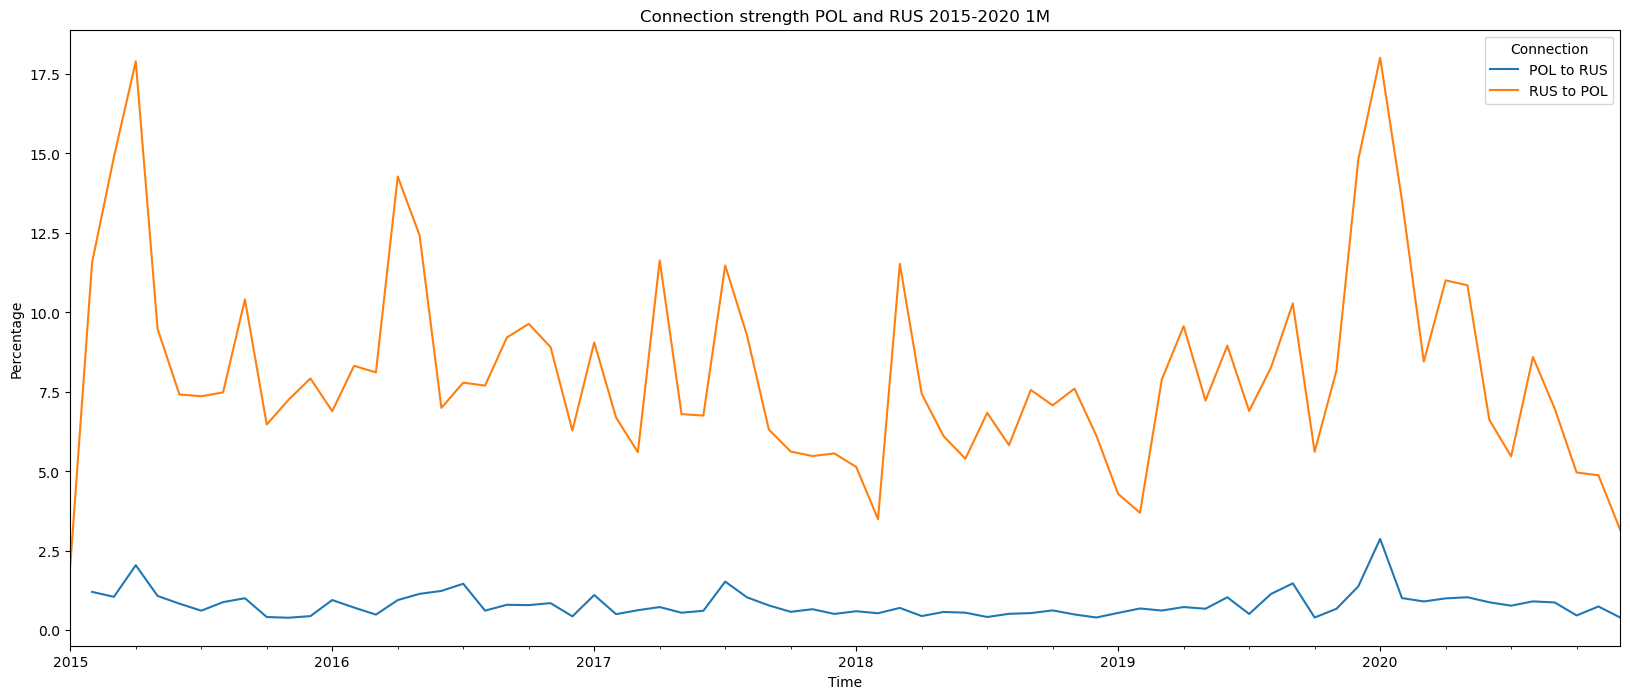
\includegraphics[width=\linewidth]{../spade_proto/figures/symmetry/POL and RUSconnection 1M.png}
        \caption{Wykres siły połączenia Polski i~Rosji. (źródło: opracowanie własne)}
        \label{fig:POL and RUS connection 1M}
    \end{figure}

    Zdarzenia są agregowane miesięcznie.
    Obserwujemy wyraźny wzrost zainteresowania Rosją przez Polskę na~początku 2020 roku.
    Taki wynik jest zgodny z~zdarzeniami ze świata rzeczywistego.
    W tym okresie odbywały się wybory parlamentarne w~Rosji.


    \section{Poszukiwanie korelacji}\label{sec:poszukiwanie-korelacji}

    \subsection{Globalna korelacja Pearsona, Kendalla oraz Spearmana}
    Wykres~\ref{fig:Connection strength pearson correlation 2015-2020} przedstawia korelację Pearsona siły połączenia miedzy parami krajów.

    \begin{figure}[!ht]
        \centering
        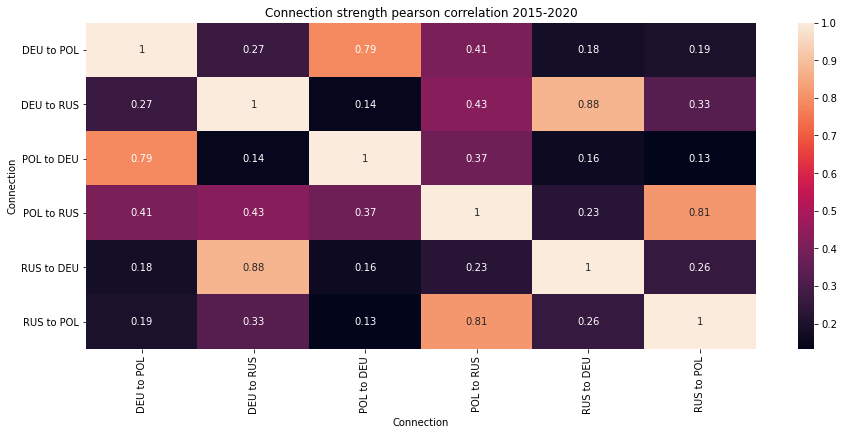
\includegraphics[width=\linewidth]{../spade_proto/figures/correlation/Connection strength pearson correlation 2015-2020.png}
        \caption{Diagram kolorów (heatmap) korelacji Pearsona siły połączenia. (źródło: opracowanie własne)}
        \label{fig:Connection strength pearson correlation 2015-2020}
    \end{figure}

    Obserwujemy wysoki (ponad 0.8) współczynnik korelacji dla przeciwnych par (jak Polska-Niemcy oraz Niemcy-Polska).
    Zauważalna (ponad 0.4) jest korelacja siły połączenia Niemiec i~Rosji oraz Polski i~Rosji.
    Wyniki te są zgodne z~intuicją.

    \begin{figure}[!ht]
        \centering
        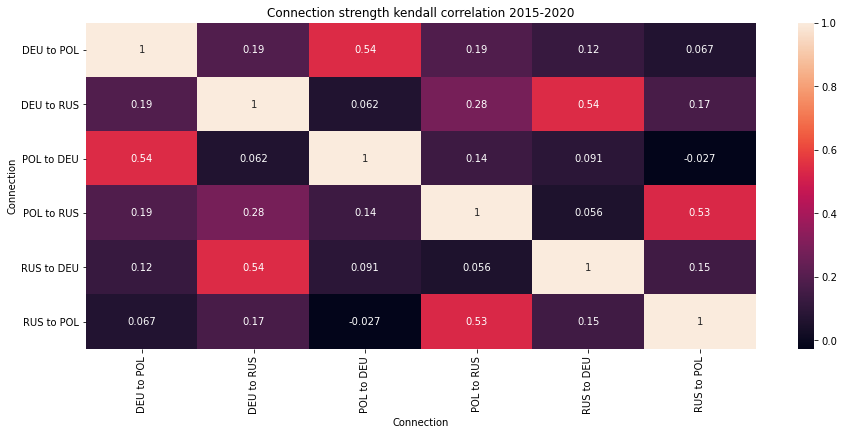
\includegraphics[width=\linewidth]{../spade_proto/figures/correlation/Connection strength kendall correlation 2015-2020.png}
        \caption{Diagram kolorów (heatmap) korelacji Kendalla siły połączenia. (źródło: opracowanie własne)}
        \label{fig:Connection strength kendall correlation 2015-2020}
    \end{figure}

    \begin{figure}[!ht]
        \centering
        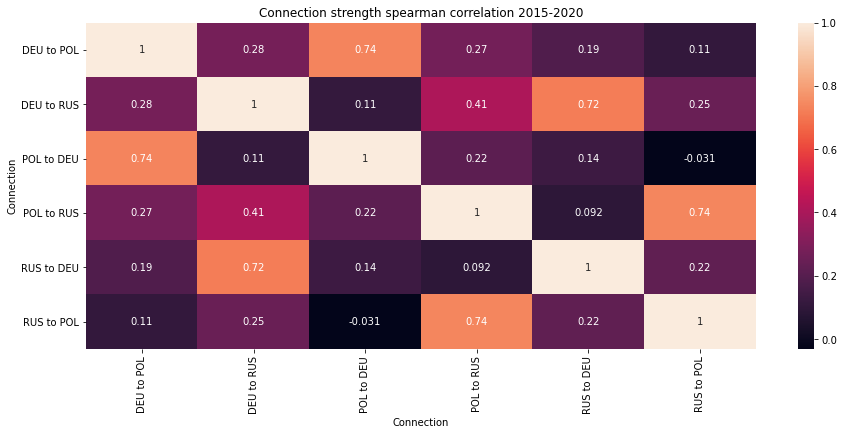
\includegraphics[width=\linewidth]{../spade_proto/figures/correlation/Connection strength spearman correlation 2015-2020.png}
        \caption{Diagram kolorów (heatmap) korelacji Spearmana siły połączenia. (źródło: opracowanie własne)}
        \label{fig:Connection strength spearman correlation 2015-2020}
    \end{figure}

    Na~wykresie przedstawiającym współczynnik korelacji Spearmana~\ref{fig:Connection strength spearman correlation 2015-2020}
    oraz Kendalla~\ref{fig:Connection strength kendall correlation 2015-2020}
    obserwujemy ujemną korelację siły połączenia Rosja-Polska i~Polska-Niemcy oraz Polska-Niemcy i~Rosja-Polska.
    Takie wyniki są zgodne z~intuicją.

    \subsection{Autokorelacja Pearsona}
    Na~dolnej osi wykresu~\ref{fig:connection-strength-pol-to-deu-autocorrelation-2015-2020} przedstawiającego
    autokorelację Pearsona dla siły połączenia Polski i~Niemiec w~latach 2015-2020 znajduje się opóźnienie w~miesiącach.

    \begin{figure}[!ht]
        \centering
        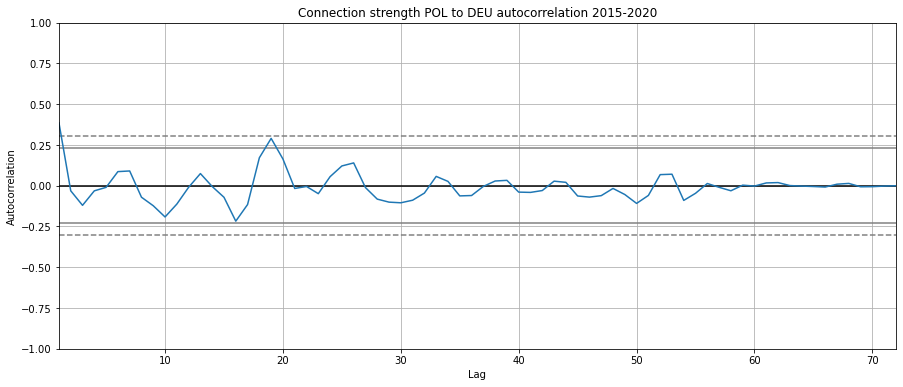
\includegraphics[width=\linewidth]{../spade_proto/figures/autocorrelation/Connection strength POL to DEU autocorrelation 2015-2020.png}
        \caption{Wykres autokorelacji siły połączenia Polski i~Niemiec. (źródło: opracowanie własne)}
        \label{fig:connection-strength-pol-to-deu-autocorrelation-2015-2020}
    \end{figure}

    Obserwujemy szczyt współczynnika korelacji około 18 miesięcy, który sugeruje powtarzalność pewnych wydarzeń co~półtora roku.

    \subsection{Korelacja Pearsona par krajów}
    Czerwonym kolorem na~wykres~\ref{fig:Connection strength DEU to POL and RUS to POL Pearson correlation with 6 months rolling 2015-2020}
    oznaczony został współczynnik korelacji siły połączenia Niemiec i~Polski oraz Rosji i~Polski (wartości na~lewej osi).
    Dodatkowo kolorem niebieskim oznaczona została siła połączenia Niemiec i~Polski, a~pomarańczowym siła połączenia Rosji i~Polski (wartości na~prawej osi).
    Dane są agregowane w~trzymiesięcznych okresach.

    \begin{figure}[!ht]
        \centering
        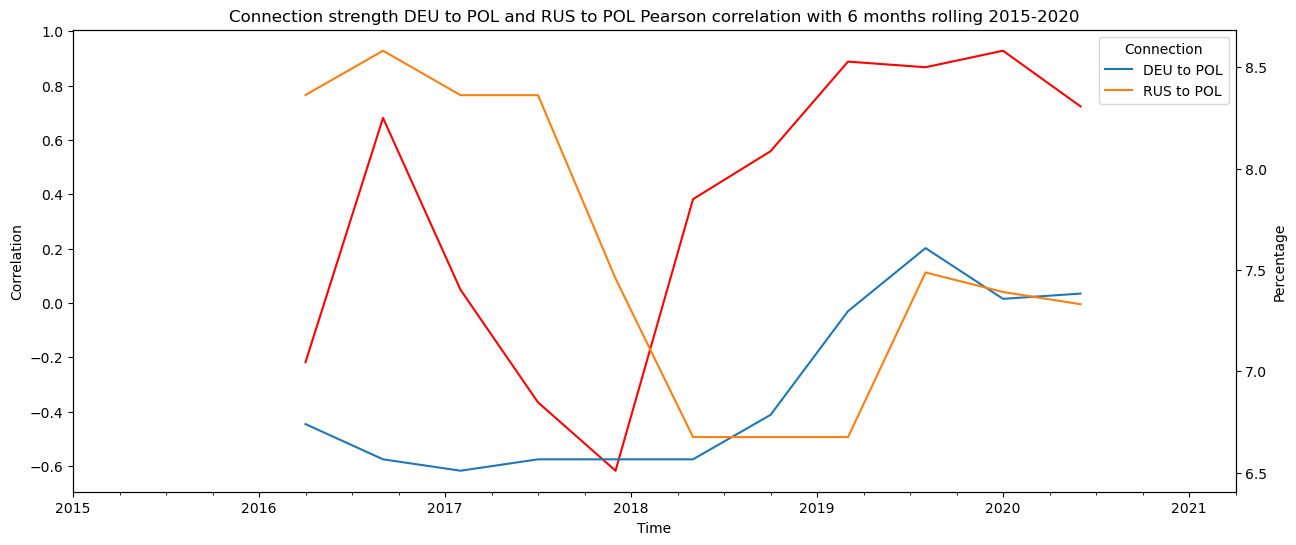
\includegraphics[width=\linewidth]{../spade_proto/figures/auto_seek/connection strength/pairwise_rolling_correlation/Connection strength DEU to POL and RUS to POL Pearson correlation with 6 months rolling 2015-2020.png}
        \caption{Wykres korelacji Pearsona siły połączenia Niemcy-Polska i~Rosja-Polska z~sześciomiesięcznym ruchomym oknem. (źródło: opracowanie własne)}
        \label{fig:Connection strength DEU to POL and RUS to POL Pearson correlation with 6 months rolling 2015-2020}
    \end{figure}

    Pierwszy wzrost współczynnika korelacji obserwujemy w~okolicach połowy 2016 roku.
    W dniu 29 lipca 2016 roku papież Franciszek przekroczył bramę ze znakiem Arbeit macht frei odwiedzając
    były obóz koncentracyjny Auschwitz-Birkenau.
    W dniu 16 września 2016 roku odbyły się wybory parlamentarne w~Rosji które wygrała partia Jedna Rosja.
    W dniach 8-9 lipca 2016 roku odbył się szczyt NATO w~Warszawie.
    Wyraźne zainteresowanie przez Polskę Niemcami oraz Rosją w~tym okresie jest zgodne z~intuicją.

    \subsection{Korelacja krzyżowa Pearsona}
    Wykres~\ref{fig:Connection strength DEU to POL and POL to DEU Pearson cross correlation 2015-2020} przedstawia korelację krzyżową siły połączenia połączenia Niemiec i~Polski oraz Polski i~Niemiec w~latach 2015-2020.

    \begin{figure}[!ht]
        \centering
        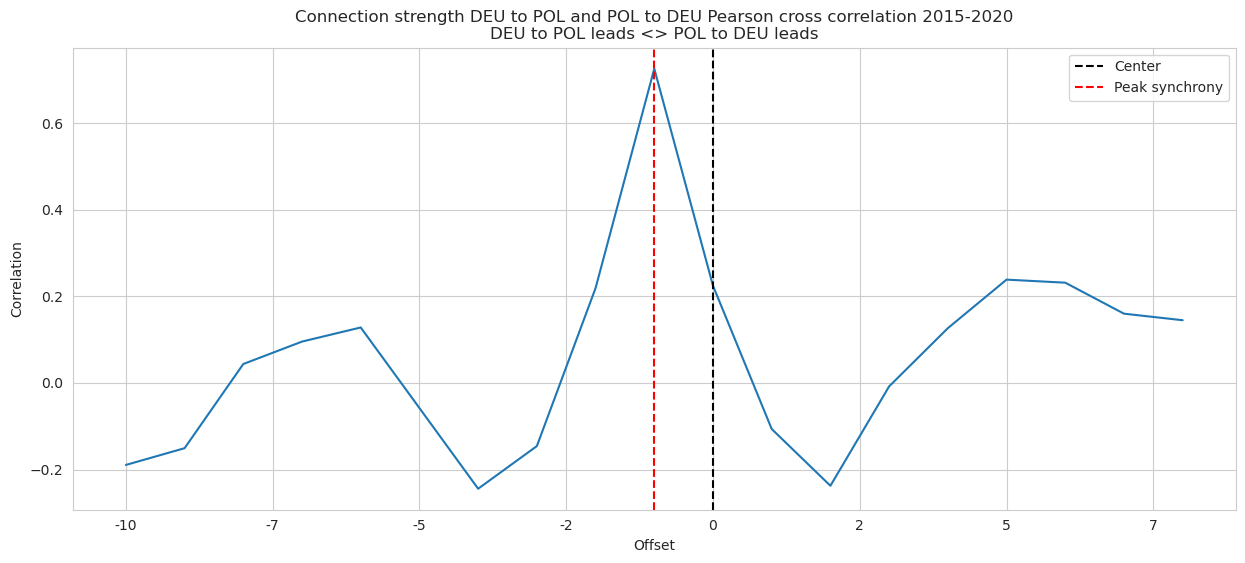
\includegraphics[width=\linewidth]{../spade_proto/figures/auto_seek/connection strength/cross_correlation/Connection strength DEU to POL and POL to DEU Pearson cross correlation 2015-2020 1M.png}
        \caption{Wykres korelacji krzyżowej Pearsona siły połączenia
        Niemcy-Polska i~Polska-Niemcy. (źródło: opracowanie własne)}
        \label{fig:Connection strength DEU to POL and POL to DEU Pearson cross correlation 2015-2020}
    \end{figure}

    Szczytowa korelacja w~około -1 miesięcznym przemieszczeniu oznacza, że zmiana znaczenia Niemiec dla Polski pociąga za sobą zmianę znaczenia Polski dla Niemiec.
    Obserwacja ta jest zgodna z~intuicją.


    \section{Klastrowanie}\label{sec:klastrowanie}
    Na~podstawie miar wybranych w~sekcji~\ref{subsec:event-base-code} przeprowadzono klastrowanie.
    Przed klastrowaniem dane poddane zostały standaryzacji poprzez usunięcie średniej i~skalowanie do~wariancji jednostkowej.
    Klastrowanie zostało przeprowadzone na~trzech grupach krajów o~znanej specyfice:
    \begin{itemize}
        \item Polska oraz Białoruś, Czechy, Niemcy, Hiszpania, Węgry, Włochy, Litwa, Rosja, Słowacja, Ukraina, Stany Zjednoczone,
        \item Tajwan oraz Chiny, Japonia, Korea Północna, Korea Południowa, Rosja, Stany Zjednoczone,
        \item Syria oraz Iran, Irak, Izrael, Rosja, Turcja, Stany Zjednoczone.
    \end{itemize}

    \subsection{Polska}
    Wyniki klastrowania aglomeracyjnego zostały przedstawione w~tabeli~\ref{tab:cluster_pl_agg}.

    \begin{table}[tp]
        \centering
        \includegraphics[width=\linewidth]{../Power-Client pre analysis/cluster_pl_agg.png}
        \caption{Wyniki klastrowania aglomeracyjnego - Polska. (źródło: opracowanie własne)}
        \label{tab:cluster_pl_agg}
    \end{table}

    Najbardziej zadowalające wyniki to~te dla punktu odcięcia równego 3 (przedostatnie z~prawej strony).
    W tym klastrowaniu relacje (1) Polski ze Stanami Zjednoczonymi, Rosją oraz Niemcami znalazły się w~jednej grupie,
    co~jest zgodne z~intuicją.
    Możemy określić relacje w~tej grupie jako Klient-Hegemon.
    Kolejna wyróżniająca się w~tym klastrowaniu grupa (0) składa z~relacji Polski z~Czechami, Węgrami, Litwą i~Słowacją.
    Możemy określić relacje w~tej grupie jako Neutralne.

    Na~wykresie~\ref{fig:cluster_pl_agg_dendrogram} przedstawiony został dendrogram do~klastrowania aglomeracyjnego.

    \begin{figure}[tp]
        \centering
        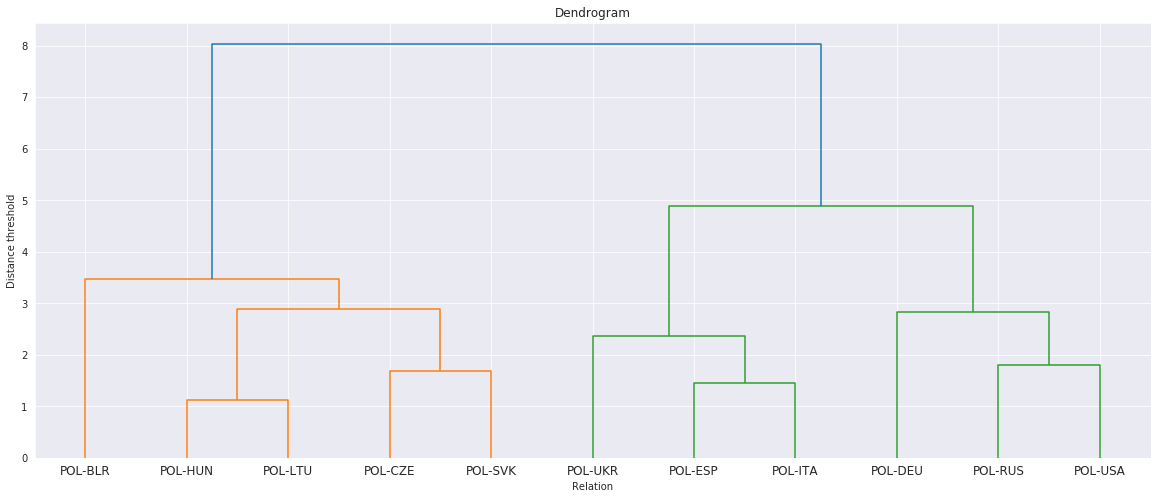
\includegraphics[width=\linewidth]{../Power-Client pre analysis/cluster_pl_agg_dendrogram.png}
        \caption{Wyniki klastrowania aglomeracyjnego - Polska. (źródło: opracowanie własne)}
        \label{fig:cluster_pl_agg_dendrogram}
    \end{figure}

    Zastanawiające jest połączenie w~jedną grupę relacji Polska-Ukraina oraz Polska-Hiszpania i~Polska-Włochy.
    Wszystkie z~pierwszych powstałych grup, widocznych u dołu dendrogramu, są zgodne z~rzeczywistymi relacjami krajów.

    W tabeli~\ref{tab:cluster_pl} przedstawione zostały wyniki klastrowania metodą kMeans.

    \begin{table}[tp]
        \centering
        \includegraphics[width=\linewidth]{../Power-Client pre analysis/cluster_pl.png}
        \caption{Wyniki klastrowania. (źródło: opracowanie własne)}
        \label{tab:cluster_pl}
    \end{table}

    Najciekawsze wydają się wyniki dla 5 klastrów, gdzie relacje Polski z~Niemcami, Rosją i~Stanami Zjednoczonymi znalazły się w~jednym klastrze.
    Tabele przedstawiające krańcowe wartości miar w~klastrowaniu k-means dla poszczególnych klastrów znajdują się w~dodatku~\ref{subsec:wartości-miar-w-klastrowaniu-kmeans---polska}.
    Wykresy gęstości miar w~poszczególnych klastrach zostały przedstawione w~dodatku~\ref{subsec:gęstośc-miar-w-poszczególnych-klastrach---polska}.

    \subsection{Tajwan}
    W tabeli~\ref{tab:cluster_tjw_agg} przedstawione zostały wyniki klastrowania aglomeracyjnego.

    \begin{table}[tp]
        \centering
        \includegraphics[width=\linewidth]{../Power-Client pre analysis/cluster_tjw_agg.png}
        \caption{Wyniki klastrowania aglomeracyjnego - Tajwan. (źródło: opracowanie własne)}
        \label{tab:cluster_tjw_agg}
    \end{table}

    Wynik dla punktu odcięcia równego 4 są najciekawsze.
    Podczas klastrowania z~tym parametrem powstały ciekawe grupy relacji:
    \begin{itemize}
        \item (0) Tajwan-Chiny, Tajwan-Rosja, Tajwan-Stany Zjednoczone,
        \item (1) Tajwan-Japonia, Tajwan-Korea Południowa,
        \item (2) Tajwan-Korea Północna.
    \end{itemize}


    Dendrogram~\ref{fig:cluster_tjw_agg_dendrogram} wyraźnie pokazuje odmienność relacji Tajwan-Korea Północna od~pozostałych,
    co~jest zgodne ze stanem faktycznym relacji między tymi państwami.

    \begin{figure}[tp]
        \centering
        \includegraphics[width=\linewidth]{../Power-Client pre analysis/cluster_tjw_agg_dendrogram.png}
        \caption{Wyniki klastrowania aglomeracyjnego - Tajwan. (źródło: opracowanie własne)}
        \label{fig:cluster_tjw_agg_dendrogram}
    \end{figure}


    Przy klastrowaniu metodą k-średnich~\ref{tab:cluster_tjw} najciekawsze wydają się wyniki dla 3 klastrów.
    Przy takiej liczbie relacje trafiają do~grup w~ten sam sposób co~dla klastrowania aglomeracyjnego z~progiem odcięcia równym 4.

    \begin{table}[tp]
        \centering
        \includegraphics[width=\linewidth]{../Power-Client pre analysis/cluster_tjw.png}
        \caption{Wyniki klastrowania. (źródło: opracowanie własne)}
        \label{tab:cluster_tjw}
    \end{table}

    Krańcowe wartości miar w~poszczególnych klastrach przedstawione są w~tabelach
    znajdujących się w~dodatku~\ref{subsec:wartości-miar-w-klastrowaniu-kmeans---tajwan}.

    Wykresy gęstości miar w~poszczególnych klastrach znalazły się w~dodatku~\ref{subsec:gęstośc-miar-w-poszczególnych-klastrach---tajwan}.

    \subsection{Syria}

    Spośród wyników klastrowania aglomeracyjnego przedstawionych w~tabeli~\ref{tab:cluster_tjw_agg} najbardziej pożądane wydają się
    te dla progów 3 i~4.

    \begin{table}[tp]
        \centering
        \includegraphics[width=\linewidth]{../Power-Client pre analysis/cluster_syr_agg.png}
        \caption{Wyniki klastrowania aglomeracyjnego - Syria. (źródło: opracowanie własne)}
        \label{tab:cluster_syr_agg}
    \end{table}

    W tym przypadku w~jednej grupie (2) znalazły się relacje wrogie Syria-Irak oraz Syria-Izrael.
    W kolejnej grupie (0) są relacje Syria-Turcja oraz Syria-Stany Zjednoczone.
    Możemy określić te relacje jako Klient-Hegemon.


    Na~wykresie~\ref{fig:cluster_syr_agg_dendrogram} przedstawiającym dendrogram obserwujemy, że relacje
    Syria-Turcja i~Syria-Stany Zjednoczone są wyraźnie oddalone od~pozostałych.

    \begin{figure}[tp]
        \centering
        \includegraphics[width=\linewidth]{../Power-Client pre analysis/cluster_syr_agg_dendrogram.png}
        \caption{Wyniki klastrowania aglomeracyjnego - Syria. (źródło: opracowanie własne)}
        \label{fig:cluster_syr_agg_dendrogram}
    \end{figure}

    Metoda k-średnich daje najlepsze wyniki, przedstawione w~tabeli ~\ref{tab:cluster_syr}, dla 3 klastrów.

    \begin{table}[tp]
        \centering
        \includegraphics[width=\linewidth]{../Power-Client pre analysis/cluster_syr_kmeans.png}
        \caption{Wyniki klastrowania. (źródło: opracowanie własne)}
        \label{tab:cluster_syr}
    \end{table}

    Przy tej konfiguracji ponownie w~tej samej grupie znalazły się relacje wrogie Syria-Irak oraz Syria-Izrael.

    W dodatku~\ref{subsec:wartości-miar-w-klastrowaniu-kmeans---syria} znalazły się tabele przedstawiające krańcowe wartości miar w~poszczególnych klastrach.

    Gęstości miar w~poszczególnych klastrach zostały przedstawione na~wykresach w~dodatku~\ref{subsec:gęstośc-miar-w-poszczególnych-klastrach---syria}.


    \chapter{Podsumowanie}\label{ch:podsumowanie}


    \section{Wnioski}\label{sec:wnioski}
    Przeprowadzone badania pokazują, że siła połączenia pomiędzy parami krajów dobrze odzwierciedla ich wzajemne zainteresowanie.
    Czas w~którym zachodzą gwałtowne zmiany siły połączenia może być dobrym punktem do~dalszych eksploracji.

    Badanie korelacji siły połączenia przyniosło zadowalające rezultaty dla każdego z~analizowanych rodzajów korelacji:
    \begin{itemize}
        \item korelacja Pearsona, Kendalla oraz Spearmana,
        \item autokorelacja Pearsona,
        \item korelacja Pearsona dla par krajów,
        \item korelacja krzyżowa Pearsona.
    \end{itemize}

    Zgodne z~oczekiwaniami są też efekty klastrowania krajów w~poszukiwaniu relacji klient-hegemon.
    Wybór w~analizie Power-Client miar do~klastrowania okazał się właściwy.
    W każdej z~trzech analizowanych grup krajów udało się zidentyfikować klaster relacji klient-hegemon oraz klaster relacji neutralnych.

    Otrzymane wynik wskazują na~duży potencjał drzemiący w~bazie danych GDELT\@.
    W trakcie pracy pojawiało się wiele interesujących wątków i~pomysłów na~dalsze badania, niestety wykraczające poza ramy tego opracowania.
    Część z~nich została opisana w~sekcji~\ref{sec:dalsze-kierunki-rozwoju}.
    Wiele z~wykresów uzyskanych podczas automatycznej eksploracji z~wykorzystaniem systemu agentowego nie zostało poddanych wnikliwej analizie
    ani przedstawionych w~tej pracy ze względu na~ograniczenia czasowe.
    Cele pracy~\ref{sec:cele-pracy} którymi były aliza wydarzeń politycznych i~poszukiwanie wzorców zostały osiągnięte.
    Zaproponowany system agentowy jest dobrą podstawą do~dalszego rozwoju i~stwarza wiele możliwości szerszej eksploracji danych z~GDELT\@.


    \section{Dalsze kierunki rozwoju}\label{sec:dalsze-kierunki-rozwoju}
    Poniżej przedstawiono propozycje dalszych kierunków rozwoju pracy.

    System Agentowy można rozbudować o~kolejne typy agentów np.: szukające wzorców w~danych Banku Światowego.
    Dodanie agentów dedykowanych poszukiwaniu wzorców wewnątrz kraju pozwoli na~wcześniejsze odrzucenie relacji niepożądanych.
    Dodanie elementów uczenia maszynowego poskutkuje zwiększeniem autonomii agentów.
    Wprowadzenie nowych progów miar pozwoli na~odrzucenie poszukiwań w~mało interesujących obszarach.
    Zarówno w~odniesieniu do~krajów jak i~relacji możliwe jest badanie przynależności do~klastrów w~czasie.

    Dostosowanie systemu może pozwolić na~analizę aktywności rynków giełdowych oraz zachowań w~mediach społecznościowych.


    \inputencoding{utf8}
    \newpage
    \addcontentsline{toc}{chapter}{Bibliografia}
    \printbibliography[title={Bibliografia}]

    \appendix
    \newpage


    \chapter{Instalacja platformy wieloagentowej}


    \section{Prosody}
    Do działania platformy SPADE niezbędny jest serwer XMPP\@.
    Przykładem takiego oprogramowania na~licencji otwarto-źródłowej jest Prosody.
    Prosody~\cite{prosody} jest nowoczesnym serwerem komunikacyjnym XMPP\@.
    W celu jego instalacji w~systemie operacyjnym Linux Debian lub Ubuntu należy skorzystać z~polecenia:
    \begin{verbatim}
           sudo apt-get install prosody
    \end{verbatim}

    Dodanie użytkownika następuje przez wydanie polecenia:
    \begin{verbatim}
        sudo prosodyctl adduser me@localhost
    \end{verbatim}

    Aby zezwolić użytkownikom na~rejestrację nowych kont i~zmianę haseł należy edytować plik:
    \begin{verbatim}
        /etc/prosody/prosody.cfg.lua
    \end{verbatim}
    zmieniając na: \textit{allow\_registration = true;}
    Następnie należy zrestartować program Prosody używając polecenia:
    \begin{verbatim}
        sudo /etc/init.d/prosody restart
    \end{verbatim}.


    \section{SPADE}

    Aby zainstalować SPADE wystarczy w~terminalu wydać polecenie:
    \begin{verbatim}
        pip install spade
    \end{verbatim}

    W celu stworzenia agenta należy postępować wg instrukcji~\cite{SPADEquickstart}:
    \begin{verbatim}
    from spade import agent

    class DummyAgent(agent.Agent):
        async def setup(self):
            print("Hello World! I'm agent {}".format(str(self.jid)))

    dummy = DummyAgent("your_jid@your_xmpp_server", "your_password")
    dummy.start()

    dummy.stop()
    \end{verbatim}

    W SPADE do~tworzenia wiadomości przeznaczona jest klasa \textit{Message},
    która pozwala na~wprowadzenie metadanych do~wiadomości.
    Metadane w~postaci słowników klucz, wartość są przydatne do~uwzględnienia atrybutów FIPA\@.

    Funkcje \textbf{send} oraz \textbf{receive} są procesami asynchronicznymi dlatego należy je wywoływać z~instrukcją \textit{await}.
    Ponieważ SPADE jest platformą do~przesyłania wiadomości w~czasie rzeczywistym,
    to~wysłana wiadomość przepadnie jeśli odbiorca nie jest gotowy na~jej odebranie.
    Dzięki XMPP agenci SPADE są zdolni do~utrzymywania listy kontaktów i~mogą otrzymywać powiadomienia o~ich kontaktach w~czasie rzeczywistym.
    Ta funkcjonalność pozwala podnieść niezawodność komunikacji.


    \section{BigQuery}
    W celu zainstalowania biblioteki google cloud dla języka python należy skorzystać z~polecenia:
    \begin{verbatim}
        pip install --upgrade 'google-cloud-bigquery[bqstorage,pandas]'
    \end{verbatim}


    \section{fpdf2}
    fpdf2 to~minimalistyczna biblioteka do~tworzenia plików PDF w~Python.
    W celu zainstalowania biblioteki fpdf2 należy skorzystać z~polecenia:
    \begin{verbatim}
        pip install fpdf2
    \end{verbatim}


    \chapter{Dodatkowe wyniki}


    \section{Analiza zdarzeń wewnętrznych USA}

    \subsection{Kody bazowe (Event Base Codes)}\label{subsec:kody-bazowenullevent-base-codesnull2}
    Wykres~\ref{fig:USA_inner_EBCperc} przedstawiają procentowy udział zdarzeń wewnętrznych w~USA z~poszczególnymi kodami bazowymi.

    \begin{figure}[tp]
        \centering
        \includegraphics[width=\linewidth]{fig/USA inner/EBCperc.png}
        \caption{Procentowa liczba zdarzeń wewnętrznych USA dla kodów bazowych od~2015 - top 10. (źródło: opracowanie własne)}
        \label{fig:USA_inner_EBCperc}
    \end{figure}

    Wykres~\ref{fig:USA_not_inner_EBCperc} przedstawiają procentowy udział zdarzeń pomiędzy USA i~innymi krajami z~poszczególnymi kodami bazowymi.

    \begin{figure}[tp]
        \centering
        \includegraphics[width=\linewidth]{fig/USA not inner/EBCperc.png}
        \caption{Procentowa liczba zdarzeń zewnętrznych USA dla kodów bazowych od~2015 - top 10. (źródło: opracowanie własne)}
        \label{fig:USA_not_inner_EBCperc}
    \end{figure}

    Wykres~\ref{fig:GLOBAL_EBCperc} przedstawiają globalny procentowy udział zdarzeń z~poszczególnymi kodami bazowymi.

    \begin{figure}[tp]
        \centering
        \includegraphics[width=\linewidth]{fig/GLOBAL//EBCperc.png}
        \caption{Procentowa liczba zdarzeń dla kodów bazowych od~2015 - top 10. (źródło: opracowanie własne)}
        \label{fig:GLOBAL_EBCperc}
    \end{figure}

    \subsection{Kody podstawowe (Event Root Codes)}\label{subsec:kody-podstawowenullevent-root-codesnull2}

    Wykres~\ref{fig:USA_inner_ERCperc} przedstawiają procentowy udział zdarzeń wewnętrznych w~USA z~poszczególnymi kodami podstawowymi.

    \begin{figure}[tp]
        \centering
        \includegraphics[width=\linewidth]{fig/USA inner/ERCperc.png}
        \caption{Procentowa liczba zdarzeń wewnętrznych USA dla wszystkich kodów podstawowych od~2015. (źródło: opracowanie własne)}
        \label{fig:USA_inner_ERCperc}
    \end{figure}

    Wykres~\ref{fig:USA_not_inner_ERCperc} przedstawiają procentowy udział zdarzeń pomiędzy USA i~innymi krajami z~poszczególnymi kodami podstawowymi.

    \begin{figure}[tp]
        \centering
        \includegraphics[width=\linewidth]{fig/USA not inner/ERCperc.png}
        \caption{Procentowa liczba zdarzeń zewnętrznych USA dla kodów podstawowych od~2015 - top 10. (źródło: opracowanie własne)}
        \label{fig:USA_not_inner_ERCperc}
    \end{figure}

    Wykres~\ref{fig:GLOBAL_ERCperc} przedstawiają globalny procentowy udział zdarzeń z~poszczególnymi kodami podstawowymi.

    \begin{figure}[tp]
        \centering
        \includegraphics[width=\linewidth]{fig/GLOBAL/ERCperc.png}
        \caption{Procentowa liczba zdarzeń dla kodów podstawowych od~2015 - top 10. (źródło: opracowanie własne)}
        \label{fig:GLOBAL_ERCperc}
    \end{figure}

    \subsection{Czterokody (Quad Class)}\label{subsec:czterokodynullquad-classnull2}

    Wykres~\ref{fig:USA_inner_QCperc} przedstawiają procentowy udział zdarzeń wewnętrznych w~USA z~poszczególnymi czterokodami.

    \begin{figure}[tp]
        \centering
        \includegraphics[width=\linewidth]{fig/USA inner/QCperc.png}
        \caption{Procentowa liczba zdarzeń wewnętrznych USA dla czterokodów od~2015 - top 10. (źródło: opracowanie własne)}
        \label{fig:USA_inner_QCperc}
    \end{figure}

    Wykres~\ref{fig:USA_not_inner_QCperc} przedstawiają procentowy udział zdarzeń pomiędzy USA i~innymi krajami z~poszczególnymi czterokodami.

    \begin{figure}[tp]
        \centering
        \includegraphics[width=\linewidth]{fig/USA not inner/QCperc.png}
        \caption{Procentowa liczba zdarzeń zewnętrznych USA dla kodów podstawowych od~2015 - top 10. (źródło: opracowanie własne)}
        \label{fig:USA_not_inner_QCperc}
    \end{figure}

    Wykres~\ref{fig:GLOBAL_QCperc} przedstawiają globalny procentowy udział zdarzeń z~poszczególnymi czterokodami.

    \begin{figure}[tp]
        \centering
        \includegraphics[width=\linewidth]{fig/GLOBAL/QCperc.png}
        \caption{Procentowa liczba zdarzeń dla kodów podstawowych od~2015 - top 10. (źródło: opracowanie własne)}
        \label{fig:GLOBAL_QCperc}
    \end{figure}


    \section{Analiza Power-Client}

    \subsection{Event Root Code}

    \subsubsection{Bez progowania}\label{subsubsec:erc:bez-progowania}

    Wykresy~\ref{fig:Power-Client:ERC:POL-RUS} oraz~\ref{fig:Power-Client:ERC:POL-DEU} przedstawiają relacje klient-hegemon.

    \begin{figure}[tp]
        \centering
        \includegraphics[width=\linewidth]{../Power-Client pre analysis/fig_EventRootCode/POL-RUS EventRootCode count 2015-2020 - top 20.png}
        \caption{Procentowa liczba zdarzeń POL-RUS wg kodów głównych. (źródło: opracowanie własne)}
        \label{fig:Power-Client:ERC:POL-RUS}
    \end{figure}

    \begin{figure}[tp]
        \centering
        \includegraphics[width=\linewidth]{../Power-Client pre analysis/fig_EventRootCode/POL-DEU EventRootCode count 2015-2020 - top 20.png}
        \caption{Procentowa liczba zdarzeń POL-DEU wg kodów głównych. (źródło: opracowanie własne)}
        \label{fig:Power-Client:ERC:POL-DEU}
    \end{figure}

    Wykresy~\ref{fig:Power-Client:ERC:POL-CZE} oraz~\ref{fig:Power-Client:ERC:POL-HUN} przedstawiają relacje neutralne.

    \begin{figure}[tp]
        \centering
        \includegraphics[width=\linewidth]{../Power-Client pre analysis/fig_EventRootCode/POL-CZE EventRootCode count 2015-2020 - top 20.png}
        \caption{Procentowa liczba zdarzeń POL-CZE wg kodów głównych. (źródło: opracowanie własne)}
        \label{fig:Power-Client:ERC:POL-CZE}
    \end{figure}

    \begin{figure}[tp]
        \centering
        \includegraphics[width=\linewidth]{../Power-Client pre analysis/fig_EventRootCode/POL-HUN EventRootCode count 2015-2020 - top 20.png}
        \caption{Procentowa liczba zdarzeń POL-HUN wg kodów głównych. (źródło: opracowanie własne)}
        \label{fig:Power-Client:ERC:POL-HUN}
    \end{figure}

    \subsubsection{Próg skala Goldsteina >=3}\label{subsubsec:erc:próg-skala-goldsteina->=3}

    Wykresy~\ref{fig:Power-Client:ERC:Goldstein:POL-RUS} oraz~\ref{fig:Power-Client:ERC:Goldstein:POL-DEU} przedstawiają relacje klient-hegemon.

    \begin{figure}[tp]
        \centering
        \includegraphics[width=\linewidth]{../Power-Client pre analysis/fig_EventRootCode/POL-RUS EventRootCode count 2015-2020 with Goldstein Scale >=3 - top 20.png}
        \caption{Procentowa liczba zdarzeń POL-RUS wg kodów głównych. (źródło: opracowanie własne)}
        \label{fig:Power-Client:ERC:Goldstein:POL-RUS}
    \end{figure}

    \begin{figure}[tp]
        \centering
        \includegraphics[width=\linewidth]{../Power-Client pre analysis/fig_EventRootCode/POL-DEU EventRootCode count 2015-2020 with Goldstein Scale >=3 - top 20.png}
        \caption{Procentowa liczba zdarzeń POL-DEU wg kodów głównych. (źródło: opracowanie własne)}
        \label{fig:Power-Client:ERC:Goldstein:POL-DEU}
    \end{figure}

    Wykresy~\ref{fig:Power-Client:ERC:Goldstein:POL-CZE} oraz~\ref{fig:Power-Client:ERC:Goldstein:POL-HUN} przedstawiają relacje neutralne.


    \begin{figure}[tp]
        \centering
        \includegraphics[width=\linewidth]{../Power-Client pre analysis/fig_EventRootCode/POL-CZE EventRootCode count 2015-2020 with Goldstein Scale >=3 - top 20.png}
        \caption{Procentowa liczba zdarzeń POL-CZE wg kodów głównych. (źródło: opracowanie własne)}
        \label{fig:Power-Client:ERC:Goldstein:POL-CZE}
    \end{figure}

    \begin{figure}[tp]
        \centering
        \includegraphics[width=\linewidth]{../Power-Client pre analysis/fig_EventRootCode/POL-HUN EventRootCode count 2015-2020 with Goldstein Scale >=3 - top 20.png}
        \caption{Procentowa liczba zdarzeń POL-HUN wg kodów głównych. (źródło: opracowanie własne)}
        \label{fig:Power-Client:ERC:Goldstein:POL-HUN}
    \end{figure}

    \subsubsection{Próg ilość wzmianek >=5}\label{subsubsec:erc:próg-ilość-wzmianek->=5}
    Liczba wzmianek to~całkowita liczba wystąpień informacji o~danym zdarzeniu pośród dokumentów źródłowych.
    Pozwala określić ważność danego zdarzenia.
    Im więcej dyskusji o~danym zdarzeniu, tym bardziej prawdopodobne, że jest ono istotne.

    Wykresy~\ref{fig:Power-Client:ERC:Mentions:POL-RUS} oraz~\ref{fig:Power-Client:ERC:Mentions:POL-DEU} przedstawiają relacje klient-hegemon.

    \begin{figure}[tp]
        \centering
        \includegraphics[width=\linewidth]{../Power-Client pre analysis/fig_EventRootCode/POL-RUS EventRootCode count 2015-2020 with mentions >=5 - top 20.png}
        \caption{Procentowa liczba zdarzeń POL-RUS wg kodów głównych. (źródło: opracowanie własne)}
        \label{fig:Power-Client:ERC:Mentions:POL-RUS}
    \end{figure}

    \begin{figure}[tp]
        \centering
        \includegraphics[width=\linewidth]{../Power-Client pre analysis/fig_EventRootCode/POL-DEU EventRootCode count 2015-2020 with mentions >=5 - top 20.png}
        \caption{Procentowa liczba zdarzeń POL-DEU wg kodów głównych. (źródło: opracowanie własne)}
        \label{fig:Power-Client:ERC:Mentions:POL-DEU}
    \end{figure}

    Wykresy~\ref{fig:Power-Client:ERC:Mentions:POL-CZE} oraz~\ref{fig:Power-Client:ERC:Mentions:POL-HUN} przedstawiają relacje neutralne.

    \begin{figure}[tp]
        \centering
        \includegraphics[width=\linewidth]{../Power-Client pre analysis/fig_EventRootCode/POL-CZE EventRootCode count 2015-2020 with mentions >=5 - top 20.png}
        \caption{Procentowa liczba zdarzeń POL-CZE wg kodów głównych. (źródło: opracowanie własne)}
        \label{fig:Power-Client:ERC:Mentions:POL-CZE}
    \end{figure}

    \begin{figure}[tp]
        \centering
        \includegraphics[width=\linewidth]{../Power-Client pre analysis/fig_EventRootCode/POL-HUN EventRootCode count 2015-2020 with mentions >=5 - top 20.png}
        \caption{Procentowa liczba zdarzeń POL-HUN wg kodów głównych. (źródło: opracowanie własne)}
        \label{fig:Power-Client:ERC:Mentions:POL-HUN}
    \end{figure}

    \subsection{Event Base Code}

    \subsubsection{Bez progowania}\label{subsubsec:ebc:bez-progowania}

    Wykresy~\ref{fig:Power-Client:EBC:POL-RUS} oraz~\ref{fig:Power-Client:EBC:POL-DEU} przedstawiają relacje klient-hegemon.

    \begin{figure}[tp]
        \centering
        \includegraphics[width=\linewidth]{../Power-Client pre analysis/fig_EventBaseCode/POL-RUS EventBaseCode count 2015-2020 - top 20.png}
        \caption{Procentowa liczba zdarzeń POL-RUS wg kodów głównych. (źródło: opracowanie własne)}
        \label{fig:Power-Client:EBC:POL-RUS}
    \end{figure}

    \begin{figure}[tp]
        \centering
        \includegraphics[width=\linewidth]{../Power-Client pre analysis/fig_EventBaseCode/POL-DEU EventBaseCode count 2015-2020 - top 20.png}
        \caption{Procentowa liczba zdarzeń POL-DEU wg kodów głównych. (źródło: opracowanie własne)}
        \label{fig:Power-Client:EBC:POL-DEU}
    \end{figure}

    Wykresy~\ref{fig:Power-Client:EBC:POL-CZE} oraz~\ref{fig:Power-Client:EBC:POL-HUN} przedstawiają relacje neutralne.

    \begin{figure}[tp]
        \centering
        \includegraphics[width=\linewidth]{../Power-Client pre analysis/fig_EventBaseCode/POL-CZE EventBaseCode count 2015-2020 - top 20.png}
        \caption{Procentowa liczba zdarzeń POL-CZE wg kodów głównych. (źródło: opracowanie własne)}
        \label{fig:Power-Client:EBC:POL-CZE}
    \end{figure}

    \begin{figure}[tp]
        \centering
        \includegraphics[width=\linewidth]{../Power-Client pre analysis/fig_EventBaseCode/POL-HUN EventBaseCode count 2015-2020 - top 20.png}
        \caption{Procentowa liczba zdarzeń POL-HUN wg kodów głównych. (źródło: opracowanie własne)}
        \label{fig:Power-Client:EBC:POL-HUN}
    \end{figure}

    \subsubsection{Próg skala Goldsteina >=3}\label{subsubsec:ebc:próg-skala-goldsteina->=3}
    Wykresy~\ref{fig:Power-Client:EBC:Goldstein:POL-RUS} oraz~\ref{fig:Power-Client:EBC:Goldstein:POL-DEU} przedstawiają relacje klient-hegemon.

    \begin{figure}[tp]
        \centering
        \includegraphics[width=\linewidth]{../Power-Client pre analysis/fig_EventBaseCode/POL-RUS EventBaseCode count 2015-2020 with Goldstein Scale >=3 - top 20.png}
        \caption{Procentowa liczba zdarzeń POL-RUS wg kodów głównych. (źródło: opracowanie własne)}
        \label{fig:Power-Client:EBC:Goldstein:POL-RUS}
    \end{figure}

    \begin{figure}[tp]
        \centering
        \includegraphics[width=\linewidth]{../Power-Client pre analysis/fig_EventBaseCode/POL-DEU EventBaseCode count 2015-2020 with Goldstein Scale >=3 - top 20.png}
        \caption{Procentowa liczba zdarzeń POL-DEU wg kodów głównych. (źródło: opracowanie własne)}
        \label{fig:Power-Client:EBC:Goldstein:POL-DEU}
    \end{figure}

    Wykresy~\ref{fig:Power-Client:EBC:Goldstein:POL-CZE} oraz~\ref{fig:Power-Client:EBC:Goldstein:POL-HUN} przedstawiają relacje neutralne.

    \begin{figure}[tp]
        \centering
        \includegraphics[width=\linewidth]{../Power-Client pre analysis/fig_EventBaseCode/POL-CZE EventBaseCode count 2015-2020 with Goldstein Scale >=3 - top 20.png}
        \caption{Procentowa liczba zdarzeń POL-CZE wg kodów głównych. (źródło: opracowanie własne)}
        \label{fig:Power-Client:EBC:Goldstein:POL-CZE}
    \end{figure}

    \begin{figure}[tp]
        \centering
        \includegraphics[width=\linewidth]{../Power-Client pre analysis/fig_EventBaseCode/POL-HUN EventBaseCode count 2015-2020 with Goldstein Scale >=3 - top 20.png}
        \caption{Procentowa liczba zdarzeń POL-HUN wg kodów głównych. (źródło: opracowanie własne)}
        \label{fig:Power-Client:EBC:Goldstein:POL-HUN}
    \end{figure}

    \subsubsection{Próg ilość wzmianek >=5}\label{subsubsec:ebc:próg-ilość-wzmianek->=5}

    Wykresy~\ref{fig:Power-Client:EBC:Mentions:POL-RUS} oraz~\ref{fig:Power-Client:EBC:Mentions:POL-DEU} przedstawiają relacje klient-hegemon.

    \begin{figure}[tp]
        \centering
        \includegraphics[width=\linewidth]{../Power-Client pre analysis/fig_EventBaseCode/POL-RUS EventBaseCode count 2015-2020 with mentions >=5 - top 20.png}
        \caption{Procentowa liczba zdarzeń POL-RUS wg kodów głównych. (źródło: opracowanie własne)}
        \label{fig:Power-Client:EBC:Mentions:POL-RUS}
    \end{figure}

    \begin{figure}[tp]
        \centering
        \includegraphics[width=\linewidth]{../Power-Client pre analysis/fig_EventBaseCode/POL-DEU EventBaseCode count 2015-2020 with mentions >=5 - top 20.png}
        \caption{Procentowa liczba zdarzeń POL-DEU wg kodów głównych. (źródło: opracowanie własne)}
        \label{fig:Power-Client:EBC:Mentions:POL-DEU}
    \end{figure}

    Wykresy~\ref{fig:Power-Client:EBC:Mentions:POL-CZE} oraz~\ref{fig:Power-Client:EBC:Mentions:POL-HUN} przedstawiają relacje neutralne.

    \begin{figure}[tp]
        \centering
        \includegraphics[width=\linewidth]{../Power-Client pre analysis/fig_EventBaseCode/POL-CZE EventBaseCode count 2015-2020 with mentions >=5 - top 20.png}
        \caption{Procentowa liczba zdarzeń POL-CZE wg kodów głównych. (źródło: opracowanie własne)}
        \label{fig:Power-Client:EBC:Mentions:POL-CZE}
    \end{figure}

    \begin{figure}[tp]
        \centering
        \includegraphics[width=\linewidth]{../Power-Client pre analysis/fig_EventBaseCode/POL-HUN EventBaseCode count 2015-2020 with mentions >=5 - top 20.png}
        \caption{Procentowa liczba zdarzeń POL-HUN wg kodów głównych. (źródło: opracowanie własne)}
        \label{fig:Power-Client:EBC:Mentions:POL-HUN}
    \end{figure}

    \subsubsection{Próg ilość wzmianek >=10}\label{subsubsec:ebc:próg-ilość-wzmianek->=10}

    Wykresy~\ref{fig:Power-Client:EBC:Mentions10:POL-RUS} oraz~\ref{fig:Power-Client:EBC:Mentions10:POL-DEU} przedstawiają relacje klient-hegemon.

    \begin{figure}[tp]
        \centering
        \includegraphics[width=\linewidth]{../Power-Client pre analysis/fig_EventBaseCode/POL-RUS EventBaseCode count 2015-2020 with mentions >=10 - top 20.png}
        \caption{Procentowa liczba zdarzeń POL-RUS wg kodów głównych. (źródło: opracowanie własne)}
        \label{fig:Power-Client:EBC:Mentions10:POL-RUS}
    \end{figure}

    \begin{figure}[tp]
        \centering
        \includegraphics[width=\linewidth]{../Power-Client pre analysis/fig_EventBaseCode/POL-DEU EventBaseCode count 2015-2020 with mentions >=10 - top 20.png}
        \caption{Procentowa liczba zdarzeń POL-DEU wg kodów głównych. (źródło: opracowanie własne)}
        \label{fig:Power-Client:EBC:Mentions10:POL-DEU}
    \end{figure}

    Wykresy~\ref{fig:Power-Client:EBC:Mentions10:POL-CZE} oraz~\ref{fig:Power-Client:EBC:Mentions10:POL-HUN} przedstawiają relacje neutralne.

    \begin{figure}[tp]
        \centering
        \includegraphics[width=\linewidth]{../Power-Client pre analysis/fig_EventBaseCode/POL-CZE EventBaseCode count 2015-2020 with mentions >=10 - top 20.png}
        \caption{Procentowa liczba zdarzeń POL-CZE wg kodów głównych. (źródło: opracowanie własne)}
        \label{fig:Power-Client:EBC:Mentions10:POL-CZE}
    \end{figure}

    \begin{figure}[tp]
        \centering
        \includegraphics[width=\linewidth]{../Power-Client pre analysis/fig_EventBaseCode/POL-HUN EventBaseCode count 2015-2020 with mentions >=10 - top 20.png}
        \caption{Procentowa liczba zdarzeń POL-HUN wg kodów głównych. (źródło: opracowanie własne)}
        \label{fig:Power-Client:EBC:Mentions10:POL-HUN}
    \end{figure}

    \subsubsection{Próg średniego tonu >=10 lub <=-10}\label{subsubsec:ebc:próg-średniego-tonu->=10-lub-<=-10}

    Wykresy~\ref{fig:Power-Client:EBC:AvgToone10:POL-RUS} oraz~\ref{fig:Power-Client:EBC:AvgToone10:POL-DEU} przedstawiają relacje klient-hegemon.

    \begin{figure}[tp]
        \centering
        \includegraphics[width=\linewidth]{../Power-Client pre analysis/fig_EventBaseCode/POL-RUS EventBaseCode count 2015-2020 with AvgTone >=10 or AvgTone <=-10 - top 20.png}
        \caption{Procentowa liczba zdarzeń POL-RUS wg kodów głównych. (źródło: opracowanie własne)}
        \label{fig:Power-Client:EBC:AvgToone10:POL-RUS}
    \end{figure}

    \begin{figure}[tp]
        \centering
        \includegraphics[width=\linewidth]{../Power-Client pre analysis/fig_EventBaseCode/POL-DEU EventBaseCode count 2015-2020 with AvgTone >=10 or AvgTone <=-10 - top 20.png}
        \caption{Procentowa liczba zdarzeń POL-DEU wg kodów głównych. (źródło: opracowanie własne)}
        \label{fig:Power-Client:EBC:AvgToone10:POL-DEU}
    \end{figure}

    Wykresy~\ref{fig:Power-Client:EBC:AvgToone10:POL-CZE} oraz~\ref{fig:Power-Client:EBC:AvgToone10:POL-HUN} przedstawiają relacje neutralne.

    \begin{figure}[tp]
        \centering
        \includegraphics[width=\linewidth]{../Power-Client pre analysis/fig_EventBaseCode/POL-CZE EventBaseCode count 2015-2020 with AvgTone >=10 or AvgTone <=-10 - top 20.png}
        \caption{Procentowa liczba zdarzeń POL-CZE wg kodów głównych. (źródło: opracowanie własne)}
        \label{fig:Power-Client:EBC:AvgToone10:POL-CZE}
    \end{figure}

    \begin{figure}[tp]
        \centering
        \includegraphics[width=\linewidth]{../Power-Client pre analysis/fig_EventBaseCode/POL-HUN EventBaseCode count 2015-2020 with AvgTone >=10 or AvgTone <=-10 - top 20.png}
        \caption{Procentowa liczba zdarzeń POL-HUN wg kodów głównych. (źródło: opracowanie własne)}
        \label{fig:Power-Client:EBC:AvgToone10:POL-HUN}
    \end{figure}


    \section{Krańcowe wartości miar w~klastrach Power-Client}

    \subsection{Wartości miar w~klastrowaniu kmeans - Polska}\label{subsec:wartości-miar-w-klastrowaniu-kmeans---polska}

    Tabele~\ref{tab:cluster0_measures_pl},
    ~\ref{tab:cluster1_measures_pl},
    ~\ref{tab:cluster2_measures_pl},
    ~\ref{tab:cluster3_measures_pl},
    ~\ref{tab:cluster4_measures_pl}
    przedstawiają krańcowe wartości miar w~poszczególnych klastrach.

    \begin{table}[tp]
        \centering
        \includegraphics[width=\linewidth]{../Power-Client pre analysis/cluster0_measures_pl.png}
        \caption{Wartości miar w~klastrze. (źródło: opracowanie własne)}
        \label{tab:cluster0_measures_pl}
    \end{table}

    \begin{table}[tp]
        \centering
        \includegraphics[width=\linewidth]{../Power-Client pre analysis/cluster1_measures_pl.png}
        \caption{Wartości miar w~klastrze. (źródło: opracowanie własne)}
        \label{tab:cluster1_measures_pl}
    \end{table}

    \begin{table}[tp]
        \centering
        \includegraphics[width=\linewidth]{../Power-Client pre analysis/cluster2_measures_pl.png}
        \caption{Wartości miar w~klastrze. (źródło: opracowanie własne)}
        \label{tab:cluster2_measures_pl}
    \end{table}

    \begin{table}[tp]
        \centering
        \includegraphics[width=\linewidth]{../Power-Client pre analysis/cluster3_measures_pl.png}
        \caption{Wartości miar w~klastrze. (źródło: opracowanie własne)}
        \label{tab:cluster3_measures_pl}
    \end{table}

    \begin{table}[tp]
        \centering
        \includegraphics[width=\linewidth]{../Power-Client pre analysis/cluster4_measures_pl.png}
        \caption{Wartości miar w~klastrze. (źródło: opracowanie własne)}
        \label{tab:cluster4_measures_pl}
    \end{table}

    \subsection{Wartości miar w~klastrowaniu kmeans - Tajwan}\label{subsec:wartości-miar-w-klastrowaniu-kmeans---tajwan}

    Tabele~\ref{tab:cluster0_measures_tjw},
    ~\ref{tab:cluster1_measures_tjw},
    ~\ref{tab:cluster2_measures_tjw}
    przedstawiają krańcowe wartości miar w~poszczególnych klastrach.

    \begin{table}[tp]
        \centering
        \includegraphics[width=\linewidth]{../Power-Client pre analysis/cluster0_measures_tjw.png}
        \caption{Wartości miar w~klastrze. (źródło: opracowanie własne)}
        \label{tab:cluster0_measures_tjw}
    \end{table}

    \begin{table}[tp]
        \centering
        \includegraphics[width=\linewidth]{../Power-Client pre analysis/cluster1_measures_tjw.png}
        \caption{Wartości miar w~klastrze. (źródło: opracowanie własne)}
        \label{tab:cluster1_measures_tjw}
    \end{table}

    \begin{table}[tp]
        \centering
        \includegraphics[width=\linewidth]{../Power-Client pre analysis/cluster2_measures_tjw.png}
        \caption{Wartości miar w~klastrze. (źródło: opracowanie własne)}
        \label{tab:cluster2_measures_tjw}
    \end{table}

    \subsection{Wartości miar w~klastrowaniu kmeans - Syria}\label{subsec:wartości-miar-w-klastrowaniu-kmeans---syria}

    Tabele~\ref{tab:cluster0_measures_syr},
    ~\ref{tab:cluster1_measures_syr},
    ~\ref{tab:cluster2_measures_syr}
    przedstawiają krańcowe wartości miar w~poszczególnych klastrach.

    \begin{table}[tp]
        \centering
        \includegraphics[width=\linewidth]{../Power-Client pre analysis/cluster0_measures_syr.png}
        \caption{Wartości miar w~klastrze. (źródło: opracowanie własne)}
        \label{tab:cluster0_measures_syr}
    \end{table}

    \begin{table}[tp]
        \centering
        \includegraphics[width=\linewidth]{../Power-Client pre analysis/cluster1_measures_syr.png}
        \caption{Wartości miar w~klastrze. (źródło: opracowanie własne)}
        \label{tab:cluster1_measures_syr}
    \end{table}

    \begin{table}[tp]
        \centering
        \includegraphics[width=\linewidth]{../Power-Client pre analysis/cluster2_measures_syr.png}
        \caption{Wartości miar w~klastrze. (źródło: opracowanie własne)}
        \label{tab:cluster2_measures_syr}
    \end{table}


    \section{Gęstości miar w~klastrach k-means Power-Client}

    \subsection{Gęstości miar w~poszczególnych klastrach - Polska}\label{subsec:gęstośc-miar-w-poszczególnych-klastrach---polska}
    Wykresy
    ~\ref{fig:density_Consult- not specified below_nummen>=5_pl},
    ~\ref{fig:density_Engage in negotiation_nummen>=5_pl},
    ~\ref{fig:density_Make statement- not specified below_none_pl},
    ~\ref{fig:density_Praise or endorse_nummen>=10_pl},
    ~\ref{fig:density_Return release- not specified below_goldstein>=3_pl}
    przedstawiają gęstość dla poszczególnych klastrów.

    \begin{figure}[tp]
        \centering
        \includegraphics[width=\linewidth]{../Power-Client pre analysis/density_Consult- not specified below_nummen>=5_pl.png}
        \caption{Wykres gęstości dla miary - Polska. (źródło: opracowanie własne)}
        \label{fig:density_Consult- not specified below_nummen>=5_pl}
    \end{figure}

    \begin{figure}[tp]
        \centering
        \includegraphics[width=\linewidth]{../Power-Client pre analysis/density_Engage in negotiation_nummen>=5_pl.png}
        \caption{Wykres gęstości dla miary - Polska. (źródło: opracowanie własne)}
        \label{fig:density_Engage in negotiation_nummen>=5_pl}
    \end{figure}

    \begin{figure}[tp]
        \centering
        \includegraphics[width=\linewidth]{../Power-Client pre analysis/density_Make statement- not specified below_none_pl.png}
        \caption{Wykres gęstości dla miary - Polska. (źródło: opracowanie własne)}
        \label{fig:density_Make statement- not specified below_none_pl}
    \end{figure}

    \begin{figure}[tp]
        \centering
        \includegraphics[width=\linewidth]{../Power-Client pre analysis/density_Praise or endorse_nummen>=10_pl.png}
        \caption{Wykres gęstości dla miary - Polska. (źródło: opracowanie własne)}
        \label{fig:density_Praise or endorse_nummen>=10_pl}
    \end{figure}

    \begin{figure}[tp]
        \centering
        \includegraphics[width=\linewidth]{../Power-Client pre analysis/density_Return release- not specified below_goldstein>=3_pl.png}
        \caption{Wykres gęstości dla miary - Polska. (źródło: opracowanie własne)}
        \label{fig:density_Return release- not specified below_goldstein>=3_pl}
    \end{figure}

    \subsection{Gęstości miar w~poszczególnych klastrach - Tajwan}\label{subsec:gęstośc-miar-w-poszczególnych-klastrach---tajwan}

    Wykresy
    ~\ref{fig:density_Consult- not specified below_nummen>=5_tjw},
    ~\ref{fig:density_Engage in negotiation_nummen>=5_tjw},
    ~\ref{fig:density_Make statement- not specified below_none_tjw},
    ~\ref{fig:density_Praise or endorse_nummen>=10_tjw},
    ~\ref{fig:density_Return release- not specified below_goldstein>=3_tjw}
    przedstawiają wykresy gęstości dla poszczególnych klastrów.

    \begin{figure}[tp]
        \centering
        \includegraphics[width=\linewidth]{../Power-Client pre analysis/density_Consult- not specified below_nummen>=5_tjw.png}
        \caption{Wykres gęstości dla miary - Tajwan. (źródło: opracowanie własne)}
        \label{fig:density_Consult- not specified below_nummen>=5_tjw}
    \end{figure}

    \begin{figure}[tp]
        \centering
        \includegraphics[width=\linewidth]{../Power-Client pre analysis/density_Engage in negotiation_nummen>=5_tjw.png}
        \caption{Wykres gęstości dla miary - Tajwan. (źródło: opracowanie własne)}
        \label{fig:density_Engage in negotiation_nummen>=5_tjw}
    \end{figure}

    \begin{figure}[tp]
        \centering
        \includegraphics[width=\linewidth]{../Power-Client pre analysis/density_Make statement- not specified below_none_tjw.png}
        \caption{Wykres gęstości dla miary - Tajwan. (źródło: opracowanie własne)}
        \label{fig:density_Make statement- not specified below_none_tjw}
    \end{figure}

    \begin{figure}[tp]
        \centering
        \includegraphics[width=\linewidth]{../Power-Client pre analysis/density_Praise or endorse_nummen>=10_tjw.png}
        \caption{Wykres gęstości dla miary - Tajwan. (źródło: opracowanie własne)}
        \label{fig:density_Praise or endorse_nummen>=10_tjw}
    \end{figure}

    \begin{figure}[tp]
        \centering
        \includegraphics[width=\linewidth]{../Power-Client pre analysis/density_Return release- not specified below_goldstein>=3_tjw.png}
        \caption{Wykres gęstości dla miary - Tajwan. (źródło: opracowanie własne)}
        \label{fig:density_Return release- not specified below_goldstein>=3_tjw}
    \end{figure}

    \subsection{Gęstości miar w~poszczególnych klastrach - Syria}\label{subsec:gęstośc-miar-w-poszczególnych-klastrach---syria}

    Wykresy
    ~\ref{fig:density_Consult- not specified below_nummen>=5_syr},
    ~\ref{fig:density_Engage in negotiation_nummen>=5_syr},
    ~\ref{fig:density_Make statement- not specified below_none_syr},
    ~\ref{fig:density_Praise or endorse_nummen>=10_syr},
    ~\ref{fig:density_Return release- not specified below_goldstein>=3_syr}
    przedstawiają wykresy gęstości dla poszczególnych klastrów.

    \begin{figure}[tp]
        \centering
        \includegraphics[width=\linewidth]{../Power-Client pre analysis/density_Consult- not specified below_nummen>=5_syr.png}
        \caption{Wykres gęstości dla miary - Syria. (źródło: opracowanie własne)}
        \label{fig:density_Consult- not specified below_nummen>=5_syr}
    \end{figure}

    \begin{figure}[tp]
        \centering
        \includegraphics[width=\linewidth]{../Power-Client pre analysis/density_Engage in negotiation_nummen>=5_syr.png}
        \caption{Wykres gęstości dla miary - Syria. (źródło: opracowanie własne)}
        \label{fig:density_Engage in negotiation_nummen>=5_syr}
    \end{figure}

    \begin{figure}[tp]
        \centering
        \includegraphics[width=\linewidth]{../Power-Client pre analysis/density_Make statement- not specified below_none_syr.png}
        \caption{Wykres gęstości dla miary - Syria. (źródło: opracowanie własne)}
        \label{fig:density_Make statement- not specified below_none_syr}
    \end{figure}

    \begin{figure}[tp]
        \centering
        \includegraphics[width=\linewidth]{../Power-Client pre analysis/density_Praise or endorse_nummen>=10_syr.png}
        \caption{Wykres gęstości dla miary - Syria. (źródło: opracowanie własne)}
        \label{fig:density_Praise or endorse_nummen>=10_syr}
    \end{figure}

    \begin{figure}[tp]
        \centering
        \includegraphics[width=\linewidth]{../Power-Client pre analysis/density_Return release- not specified below_goldstein>=3_syr.png}
        \caption{Wykres gęstości dla miary - Syria. (źródło: opracowanie własne)}
        \label{fig:density_Return release- not specified below_goldstein>=3_syr}
    \end{figure}

\end{document}

